\ifx\wholebook\relax \else

\documentclass[b5paper]{ctexart}
\usepackage[nomarginpar
  %, margin=.5in
]{geometry}

\addtolength{\oddsidemargin}{-0.05in}
\addtolength{\evensidemargin}{-0.05in}
\addtolength{\textwidth}{0.1in}
\usepackage[cn]{../../../prelude}

\setcounter{page}{1}

\begin{document}

\title{B树}

\author{刘新宇
\thanks{{\bfseries 刘新宇 } \newline
  Email: liuxinyu95@gmail.com \newline}
  }

\maketitle
\fi

\markboth{B树}{基本算法}

\ifx\wholebook\relax
\chapter{B树}
\numberwithin{Exercise}{chapter}
\fi

\section{简介}
\index{B树}
\label{introduction}

上一章介绍的整数前缀树利用二叉树的边来表达信息。另一种扩展二叉树的方法是将分枝数目从2增加到$k$。B树是一种自平衡的$k$叉搜索树\cite{wiki-b-tree}。它被广泛用于计算机文件系统(基于B+树,一种B树的扩展形式)和数据库系统。\cref{fig:btree-example}展示了一棵B树,我们可以观察它和二叉搜索树之间的异同。

\begin{figure}[htbp]
  \centering
  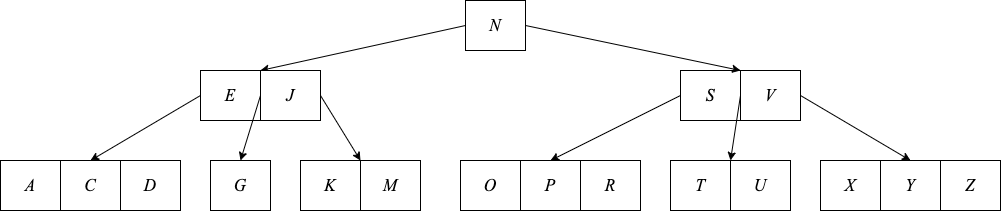
\includegraphics[scale=0.33]{img/btree-del-before}
  \caption{B树}
  \label{fig:btree-example}
\end{figure}

一棵二叉搜索树或为空,或包含一个元素$k$和左右分枝$l$、$r$。左子树$l$中的任何元素都小于$k$,并且$k$小于右子树$r$中的任何元素\footnote{严格来说,节点中可以保存键(key)和对应的值(value)。值不是必需的。简单起见,本章忽略了节点中的值,称树中保存的内容为“元素”。}:

\be
\forall\ x \in l, y \in r \Rightarrow x < k < y
\ee

B树将这一思想推广到多个分枝。一棵B树或为空,或包含$n$个元素和$n + 1$个子分枝,每个分枝也都是一棵B树。记这些元素为$k_1, k_2, ..., k_n$,分枝为$t_1, t_2, ..., t_n, t_{n+1}$,如\cref{fig:btree-node}所示。节点中的元素和分枝满足以下条件:

\begin{figure}[htbp]
  \centering
  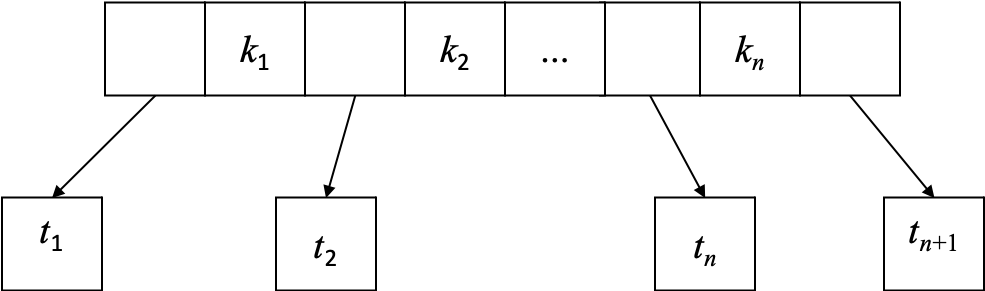
\includegraphics[scale=0.5]{img/btree-node}
  \caption{B树节点}
  \label{fig:btree-node}
\end{figure}

\begin{itemize}
\item 元素是递增的:$k_1 \leq k_2 \leq ... \leq k_n$;
\item 对于任意$k_i$,子树$t_i$中的所有元素都小于$k_i$,并且$k_i$小于子树$t_{i+1}$中的任意元素。
\end{itemize}

\begin{equation}
\forall\ x_i \in t_i, i=0, 1, ..., n\ \Rightarrow x_1 < k_1 < x_2 < k_2 < ... < x_n < k_n < x_{n+1}
\label{eq:btree-order}
\end{equation}

叶子节点不包含子分枝。令元素的类型为$K$,则B树的类型为$BTree\ K$或\texttt{BTree<K>}。此外,我们还需定义一组规则以保持B树平衡:

\begin{itemize}
\item 所有的叶子节点都有相同的深度;
\item 定义整数$d$,称为B树的\underline{最小度数},每个节点:
    \begin{itemize}
        \item 最多含有$2d - 1$个元素;
        \item 最少含有$d - 1$个元素,根节点例外。
    \end{itemize}
\end{itemize}

即:

\be
  d - 1 \leq |keys(t)|  \leq 2d - 1
\ee

我们接下来证明这些规则可以保证B树是平衡的。

\begin{proof}
考虑一棵含有$n$个元素的B树,最小度数$d \geq 2$,树的高度为$h$。除根节点外,其它节点至少含有$d - 1$个元素。根节点至少含有一个元素。如果它有子树,则至少有两个深度为1的子分枝,至少有$2d$个深度为2的子分枝,至少有$2d^2$个深度为3的子分枝……最后,至少有$2d^{h-1}$个深度为$h$的叶子节点。除根节点外,将节点个数乘以$d - 1$,B树中存储的元素个数满足下面的不等式:

\be
\begin{array}{rl}
n & \geq 1 + (d - 1)(2 + 2d + 2d^2 + ... + 2d^{h-1}) \\
  & = 1 + 2(d - 1) \displaystyle \sum_{k=0}^{h-1} d^k \\
  & = 1 + 2(d - 1) \displaystyle \frac{d^h-1}{d-1} \\
  & = 2d^h - 1
\end{array}
\ee

因此树的高度满足对数关系不等式:

\be
h \leq \log_d \frac{n+1}{2}
\ee

\end{proof}

这就证明了B树的平衡性。最简单的B树称为2-3-4树。它的最小度数$d = 2$,除根节点外的任何节点都包含2到4棵子分枝。任何红黑树本质上都可以转换为一棵2-3-4树。我们记度数为$d$的非空B树为$(d, (ks, ts))$,其中$ks$是元素列表,$ts$是子树列表。下面的例子程序定义了B树:

\lstset{frame = single}
\begin{Haskell}
data BTree a = BTree [a] [BTree a]
\end{Haskell}

空节点记为$(\nil, \nil)$或\texttt{BTree [] []},为了避免在每个节点中都存储一份$d$,我们将其和B树$t$组成一对值$(d, t)$。

\section{插入}
\index{B树!插入} \label{btree-insertion}

插入的思路和二叉搜索树类似,只不过需要处理多个元素和分枝。当向B树$t$插入元素$x$时,我们从根节点开始,查找这样的位置\footnote{实际上,元素只需支持小于比较和等于比较。参见\cref{ex:btree-leq}。}:所有左侧的元素都小于$x$,而右侧的元素大于$x$。如果是未满的叶子节点($|keys(t)| < 2d - 1$),就将$x$插入到此位置。否则,这一位置会指向一棵子树$t'$,我们递归地将$x$插入到$t'$。

\begin{figure}[htbp]
  \centering
  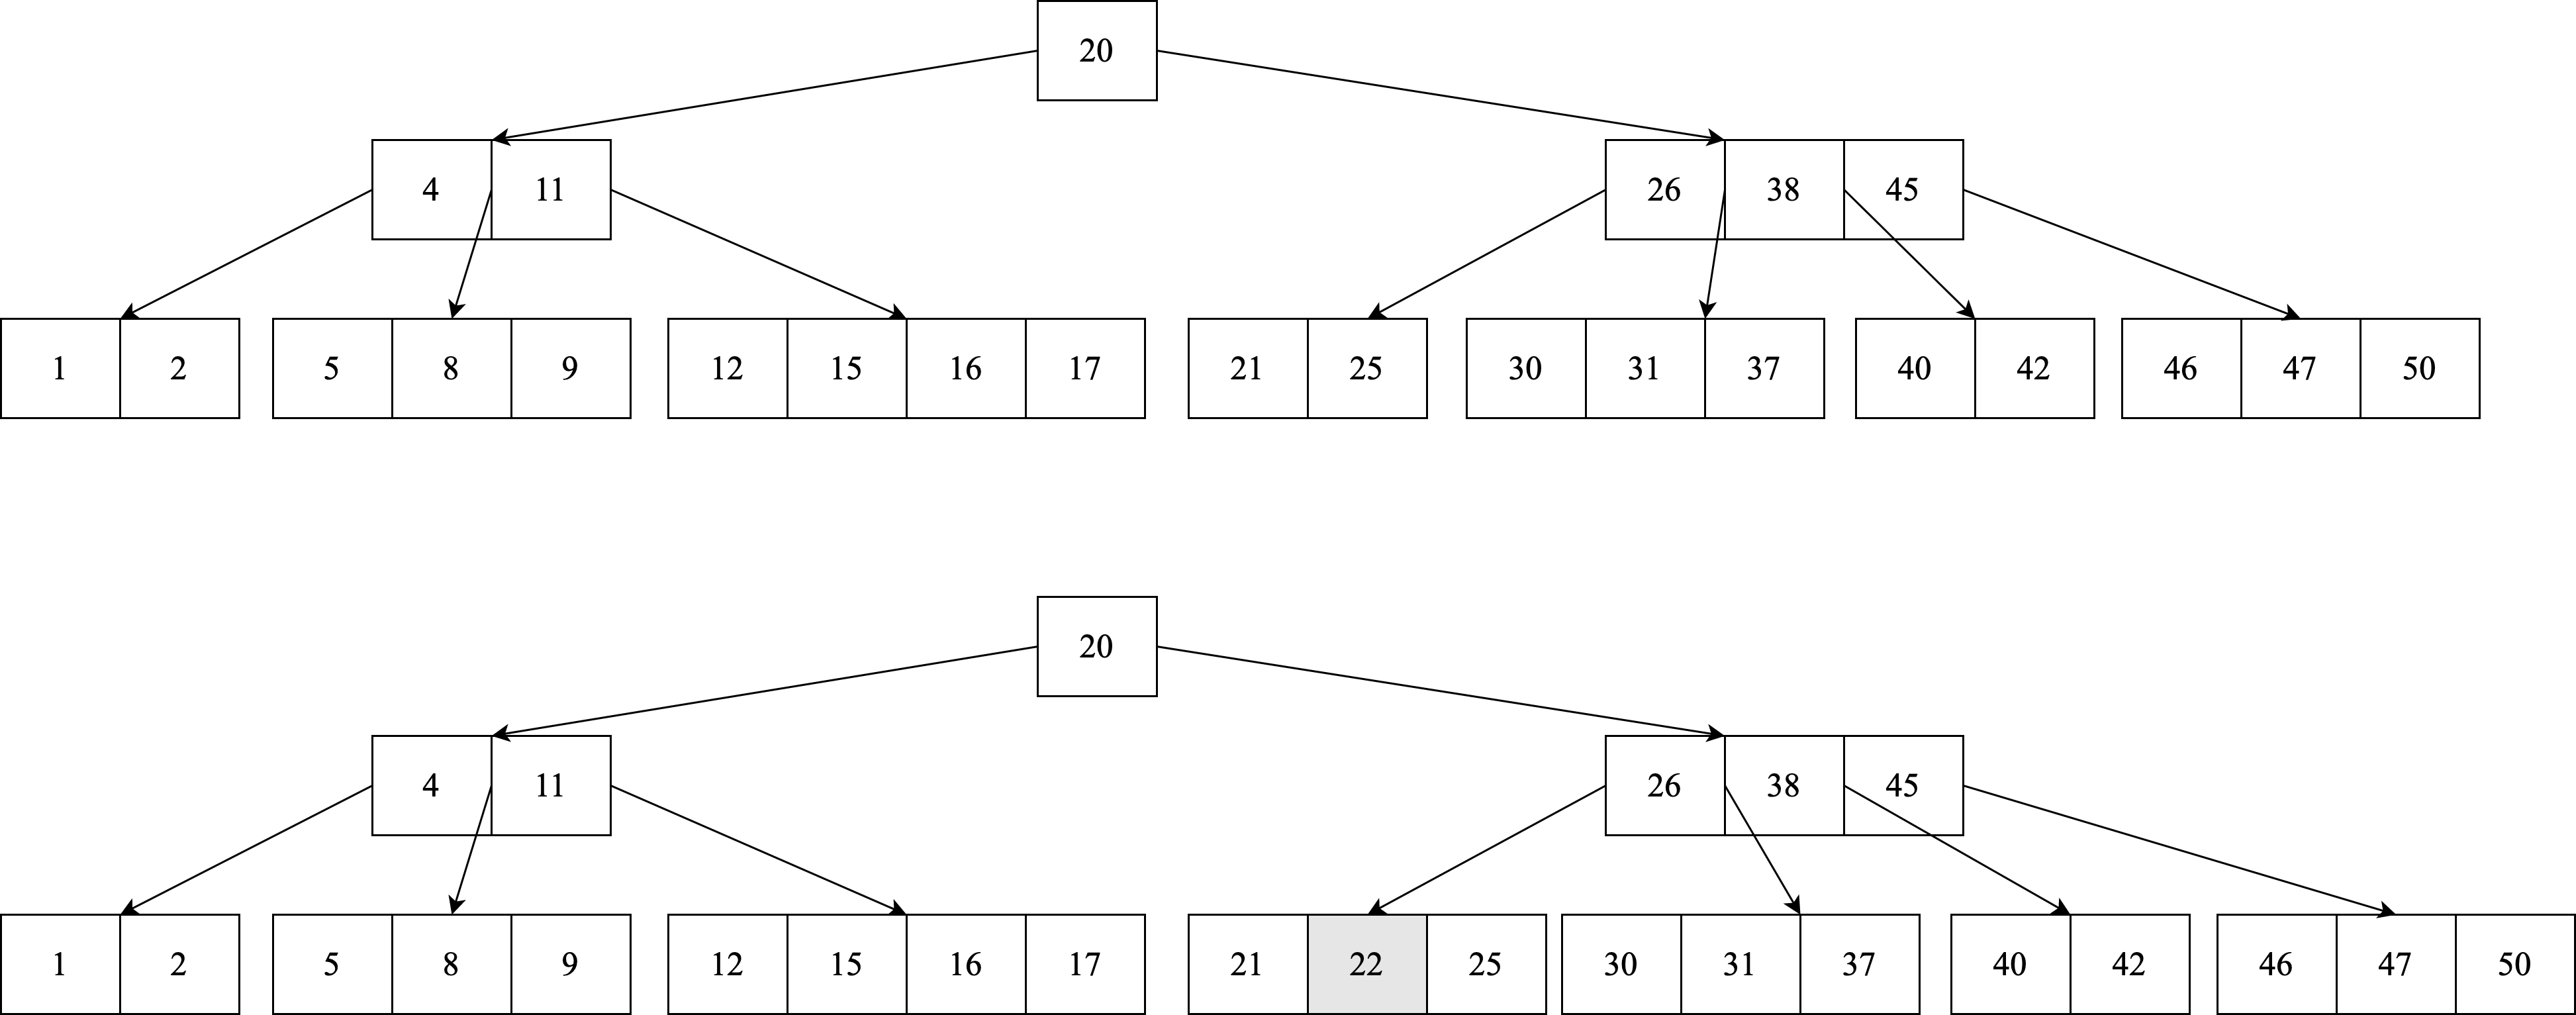
\includegraphics[scale=0.4]{img/btree-insert-example}
  \caption{将22插入到2-3-4树:$22 > 20$,插入右子树;$22 < 26$,插入第一棵子树。$21 < 22 < 25$,插入到未满的叶子节点。}
  \label{fig:btree-insert-simple}
\end{figure}

考虑向\cref{fig:btree-insert-simple}中的2-3-4树插入元素$x = 22$。因为$20 < 22$,我们转向右侧的子树。它包含26、38、45。因为$22 < 26$,所以接下来转向第一棵子树。它包含21和25。这是一个未满的叶子节点,将22插入到21和25中间。

但如果叶子节点已经含有$2d - 1$个元素,插入$x$后就会因为元素过多破坏B树的规则。例如向\cref{fig:btree-insert-simple}插入18就会遇到这个问题。我们有两种解法:先插入再分拆,和先分拆再插入。

\subsection{先插入再分拆}

我们可以将红黑树中的“先插入再修复”方法扩展到B树。先不考虑B树的平衡性,将元素插入到适当的位置。接下来,如果树不再平衡了,我们自下而上对含有过多元素的节点进行分拆。首先需要定义函数,用以判断节点是否含有过多或过少的元素。

\be
\begin{cases}
full\ d\ (ks, ts) & = |ks| > 2d - 1 \\
low\  d\ (ks, ts) & = |ks| < d - 1 \\
\end{cases}
\ee

如果含有过多元素和分枝,我们定义$split$函数将其在位置$m$分拆为三部分,如\cref{fig:node-split}所示:

\begin{figure}[htbp]
  \centering
  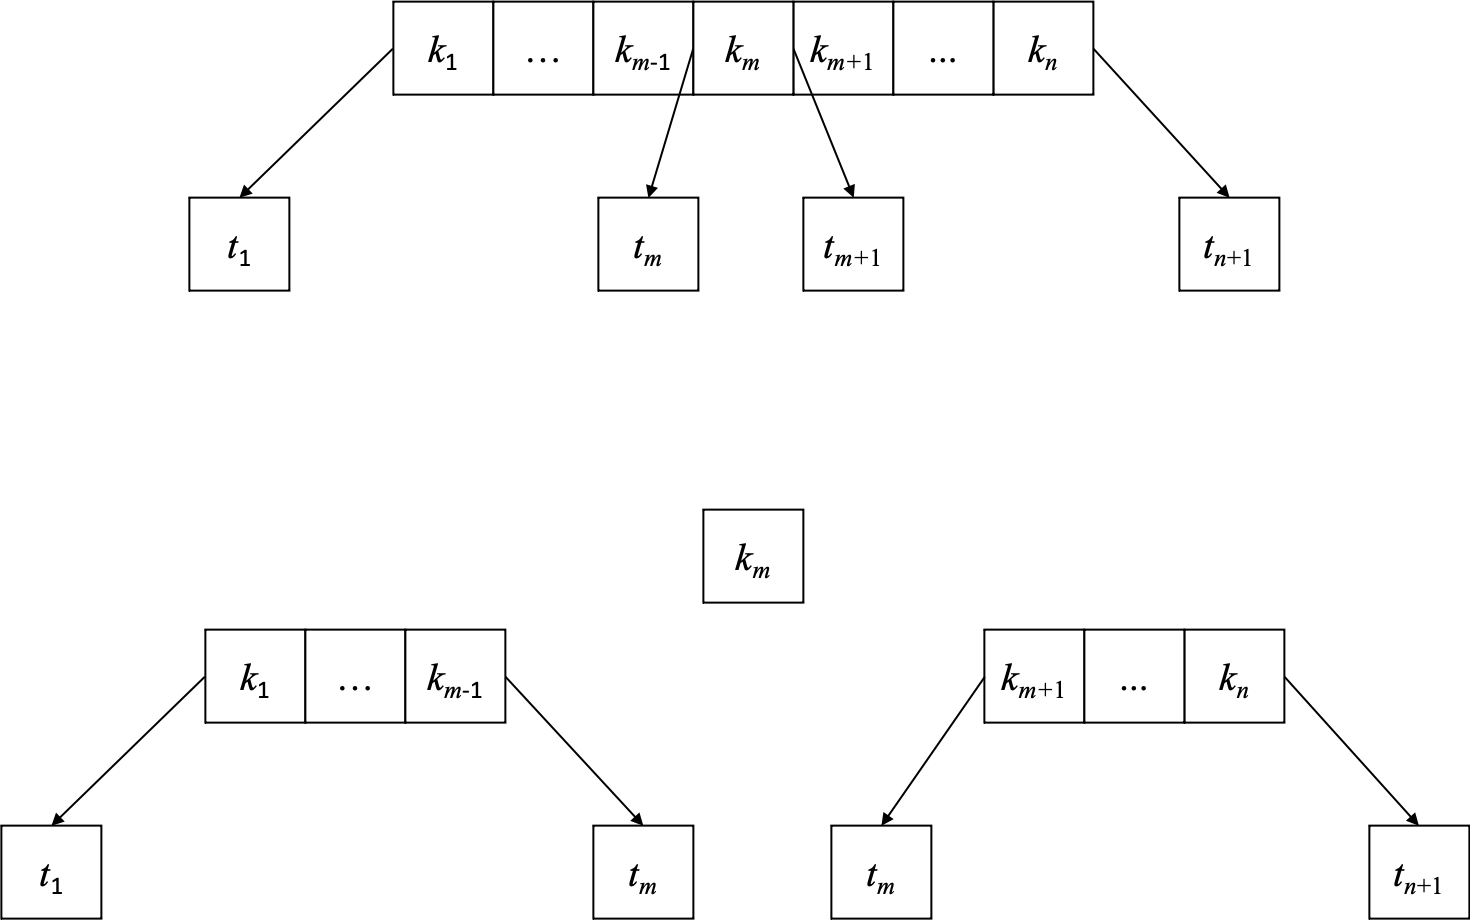
\includegraphics[scale=0.4]{img/split}
  \caption{在位置$m$将节点分拆为三部分。}
  \label{fig:node-split}
\end{figure}

\be
split\ m\ (ks, ts) = ((ks_l, ts_l), k, (ks_r, ts_r))
\ee

我们使用第一章\cref{eq:split-at}中定义的$splitAt$函数来实现:

\[
\begin{cases}
(ks_l, (k:ks_r)) & = splitAt\ (m - 1)\ ks \\
(ts_l, ts_r) & = splitAt\ m\ ts
\end{cases}
\]

对称地,我们可以定义$unsplit$函数,将三个部分合并成一个B树节点:

\be
unsplit\ (ks_l, ts_l)\ k\ (ks_r, ts_r) = (ks_l \doubleplus [k] \doubleplus ks_r, ts_l \doubleplus ts_r)
\label{eq:btree-unsplit}
\ee

下面的函数先将$x$插入树$t$,然后使用$fix$修复平衡,使其成为度数为$d$的合法B树:

\be
insert\ x\ (d, t) = fix\ (d, ins\ t)
\ee

在$ins$之后,如果根节点含有过多的元素,函数$fix$使用$split$将其分拆,并构建新的根节点。

\be
fix\ (d, t) = \begin{cases}
  full\ d\ t : & (d, ([k], [l, r])), \text{where}\ (l, k, r) = split\ d\ t \\
  otherwise  : & (d, t)
\end{cases}
\ee

函数$ins$需要处理两种情况:对于叶子节点,我们可以重用第一章\cref{eq:list-ordered-insert}定义的列表插入函数$insert$来处理;否则,我们需要找到合适的位置,递归地向子树插入。为此,我们定义函数$partition$:

\be
partition\ x\ (ks, ts) = (l, t', r)
\ee

其中$l = (ks_l, ts_l)$、$r = (ks_r, ts_r)$。它进一步使用第一章\cref{eq:span}中定义的列表函数$span$进行划分:

\[
\begin{cases}
(ks_l, ks_r) & = span\ (< x)\ ks \\
(ts_l, (t':ts_r)) & = splitAt\ |ks_l|\ ts
\end{cases}
\]

这样,所有小于$x$的元素和所在的子分枝都在左侧$l$,所有大于$x$的都在右侧$r$。我们将最后一棵小于$x$的子树取出作为$t'$。接下来我们递归地将$x$插入到$t'$中,如\cref{fig:recursive-insert}所示。

\be
\begin{array}{rcll}
  ins\ (ks, \nil) & = & (insert_L\ x\ ks, \nil) & \text{叶子节点,列表插入}\\
  ins\ (ks, ts)   & = & balance\ d\ l\ (ins\ t')\ r & \text{其中}\ (l, t', r) = partition\ x\ t \\
\end{array}
\ee

\begin{figure}[htbp]
  \centering
  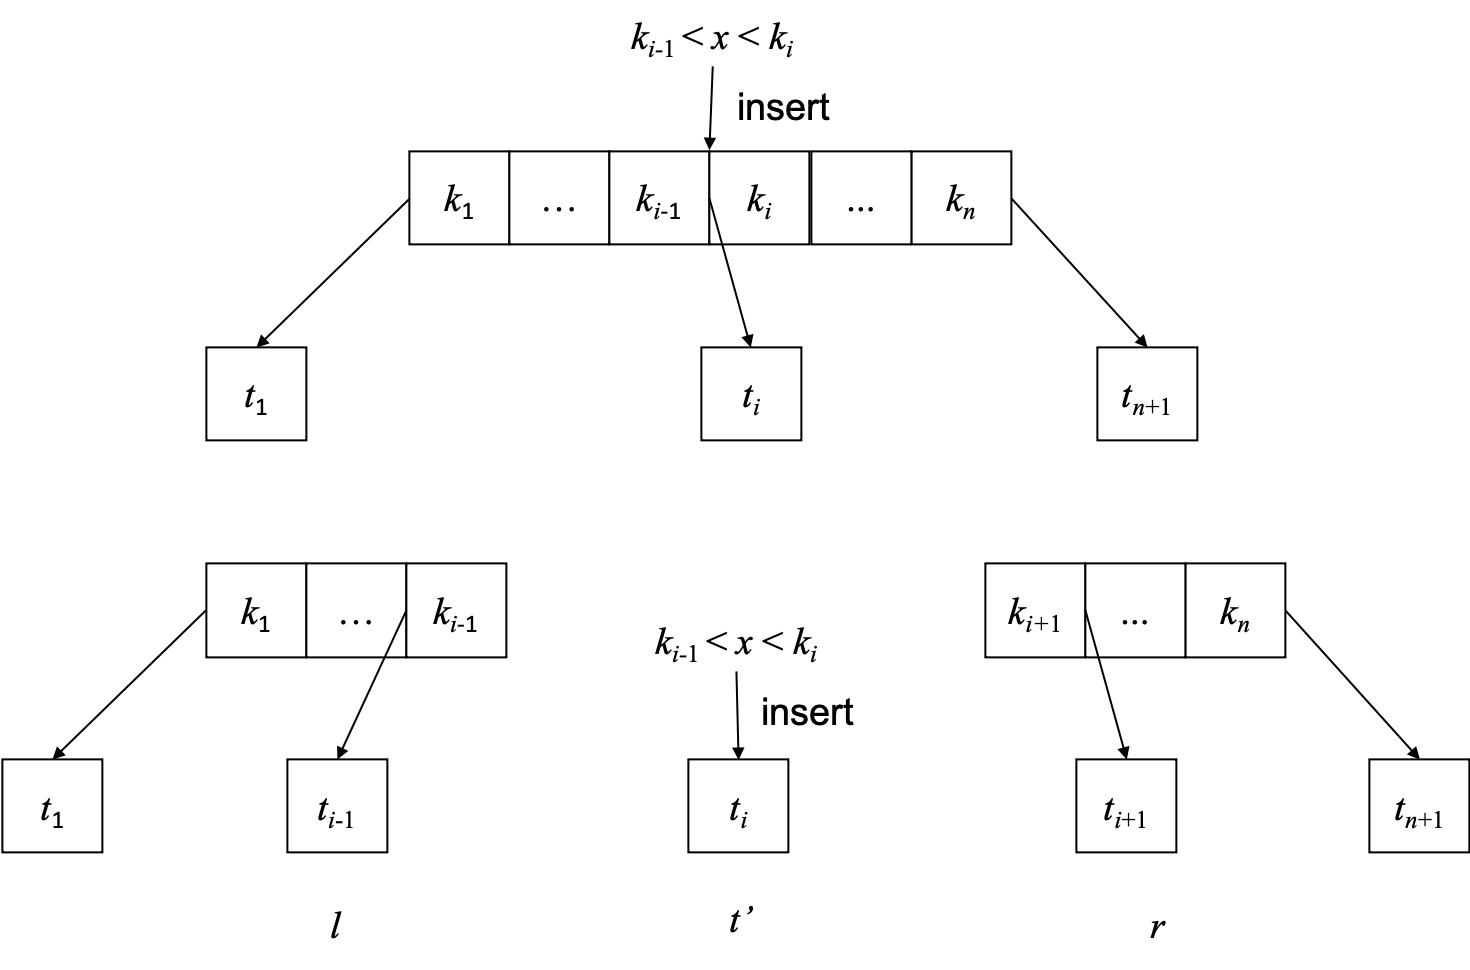
\includegraphics[scale=0.45]{img/partition}
  \caption{用$x$划分节点}
  \label{fig:recursive-insert}
\end{figure}

向$t'$插入$x$后,它可能包含过多元素,不再满足B树平衡条件。我们定义函数$balance$递归地进行分拆修复。

\be
balance\ d\ (ks_l, ts_l)\ t\ (ks_r, ts_r) = \begin{cases}
  full\ d\ t: fix_f \\
  otherwise: (ks_l \doubleplus ks_r, ts_l \doubleplus [t] \doubleplus ts_r)
  \end{cases}
\ee

其中$fix_f$将度数为$d$的子分枝$t$分拆为$(t_1, k, t_2) = split\ d\ t$,然后构建一个新的B树节点:

\be
fix_f = (ks_l \doubleplus [k] \doubleplus ks_r, ts_l \doubleplus [t_1, t_2] \doubleplus ts_r)
\ee

下面的例子程序实现了B树的插入算法:

\begin{Haskell}
partition x (BTree ks ts) = (l, t, r) where
  l = (ks1, ts1)
  r = (ks2, ts2)
  (ks1, ks2) = span (< x) ks
  (ts1, (t:ts2)) = splitAt (length ks1) ts

split d (BTree ks ts) = (BTree ks1 ts1, k, BTree ks2 ts2) where
  (ks1, k:ks2) = splitAt (d - 1) ks
  (ts1, ts2) = splitAt d ts

insert x (d, t) = fixRoot (d, ins t) where
    ins (BTree ks []) = BTree (List.insert x ks) []
    ins t = balance d l (ins t') r where (l, t', r) = partition x t

fixRoot (d, t) | full d t  = let (t1, k, t2) = split d t in
                               (d, BTree [k] [t1, t2])
               | otherwise = (d, t)

balance d (ks1, ts1) t (ks2, ts2)
    | full d t  = fixFull
    | otherwise = BTree (ks1 ++ ks2) (ts1 ++ [t] ++ ts2)
  where
    fixFull = let (t1, k, t2) = split d t in
                BTree (ks1 ++ [k] ++ ks2) (ts1 ++ [t1, t2] ++ ts2)
\end{Haskell}

\cref{fig:btree-insert-fp}给出了两棵B树的例子,它们都是依次将``GMPXACDEJKNORSTUVYZ''中的元素插入B树构造出的。

\begin{figure}[htbp]
  \centering
  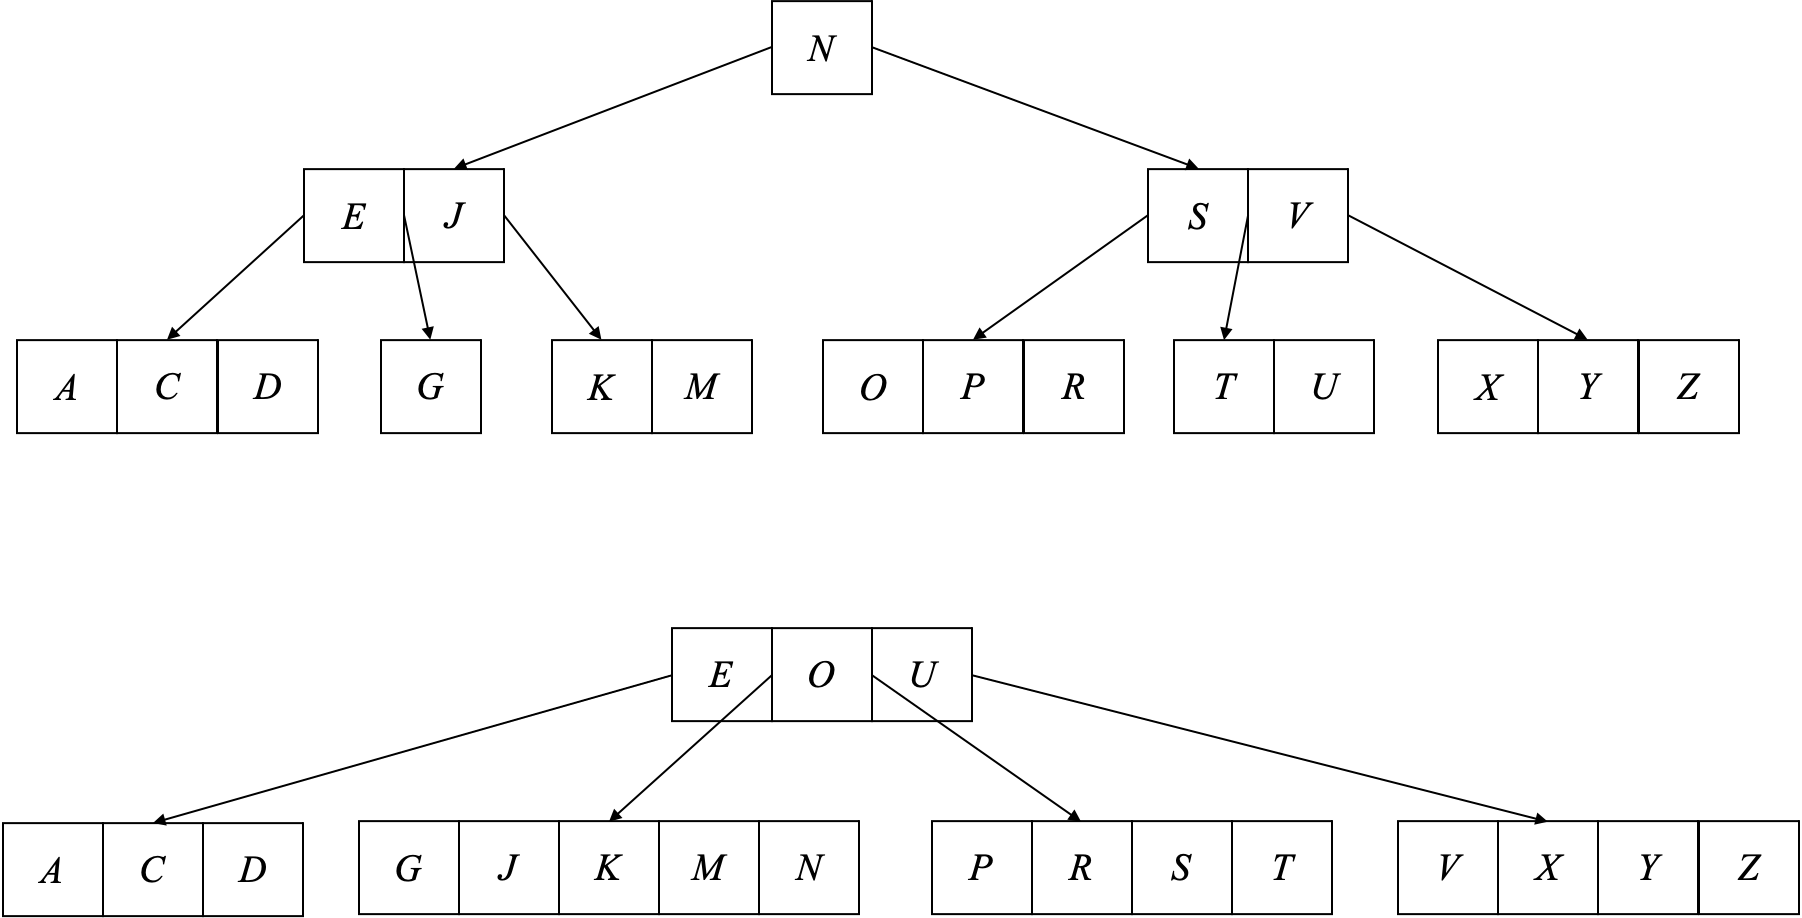
\includegraphics[scale=0.4]{img/btree-insert-fp}
  \captionsetup{justification=centering}
  \caption{依次插入``GMPXACDEJKNORSTUVYZ''。\\
上:$d = 2$(2-3-4树),下:$d = 3$}
  \label{fig:btree-insert-fp}
\end{figure}

\subsection{先分拆再插入}

第二种方法是在插入前先分拆节点以避免其含有过多元素。命令式实现常用这一方法。自顶向下递归插入时,当遇到含有$2d - 1$个元素的节点时,我们将其分拆为三部分,如\cref{fig:node-split}所示。每个新节点都只含有$d - 1$个元素,即使插入元素后也仍然是合法的B树节点。对于节点$x$,令$K(x)$表示它包含的元素,$T(x)$表示它包含的子分枝。记$x$中的第$i$个元素为$k_i(x)$,第$j$棵子分枝为$t_j(x)$。下面的算法在第$i$个位置对节点$z$进行分拆:

\begin{algorithmic}[1]
\Procedure{Split}{$z, i$}
  \State $d \gets$ \Call{Deg}{$z$}
  \State $x \gets t_i(z)$
  \State $y \gets$ \Call{Create-Node}{}
  \State $K(y) \gets [k_{d + 1}(x), k_{d + 2}(x), ..., k_{2d - 1}(x)]$
  \State $K(x) \gets [k_1(x), k_2(x), ..., k_{d-1}(x)]$
  \If{$x$ is not leaf}
    \State $T(y) \gets [t_{d + 1}(x), t_{d + 2}(x), ..., t_{2d}(x)]$
    \State $T(x) \gets [t_1(x), t_2(x), ..., t_d(x)]$
  \EndIf
  \State \Call{Insert-At}{$K(z), i, k_d(x)$}
  \State \Call{Insert-At}{$T(z), i + 1, y$}
\EndProcedure
\end{algorithmic}

分拆节点$x = t_i(z)$时,我们将第$d$个元素$k_d(x)$向上推入父节点$z$。如果$z$已经满了,推入元素后就会违反B树规则。为此,我们需要从根节点起,自顶向下沿着插入的路径进行检查,分拆所有含有$2d - 1$个元素的节点。因为所有的父节点都这样被处理过,所以可以接受推上来的元素。这一方法只需要一轮自顶向下的处理,无需回溯。如果根节点已满,则需要新建一个节点,并将原来的根节点作为它的唯一子树。下面是插入算法的实现:

\begin{algorithmic}[1]
\Function{Insert}{$t, k$}
  \State $r \gets t$
  \If{$r$ is full} \Comment{根节点已满}
    \State $s \gets$ \Call{CREATE-NODE}{}
    \State $T(s) \gets [ r ]$
    \State \Call{Split}{$s, 1$}
    \State $r \gets s$
  \EndIf
  \State \Return \Call{Insert-Nonfull}{$r, k$}
\EndFunction
\end{algorithmic}

其中算法\textproc{Insert-Nonfull}假设传入的节点$r$不满。如果$r$是叶子节点,我们按照$k$的大小将其插入到相应位置(\cref{ex:btree-binary-search}要求使用二分查找进行插入)。否则,我们找到一个位置,使得$k_i(r) < k < k_{i+1}(r)$,如果分枝$t_i(r)$满了,就进行分拆。然后继续向子分枝插入。

\begin{algorithmic}[1]
\Function{Insert-Nonfull}{$r, k$}
  \State $n \gets |K(r)|$
  \If{$r$ is leaf}
    \State $i \gets 1$
    \While{$i \leq n$ and $k > k_i(r)$}
      \State $i \gets i + 1$
    \EndWhile
    \State \Call{Insert-At}{$K(r), i, k$}
  \Else
    \State $i \gets n$
    \While{$i > 1$ and $k < k_i(r)$}
      \State $i \gets i - 1$
    \EndWhile
    \If{$t_i(r)$ is full}
      \State \Call{Split}{$r, i$}
      \If{$k > k_i(r)$}
        \State $i \gets i + 1$
      \EndIf
    \EndIf
    \State \Call{Insert-Nonfull}{$t_i(r), k$}
  \EndIf
  \State \Return $r$
\EndFunction
\end{algorithmic}

这一算法是递归的。\cref{ex:btree-loop-insert}要求使用循环消除递归。\cref{fig:btree-insert}给出了依次插入``GMPXACDEJKNORSTUVYZ''时的结果。

\begin{figure}[htbp]
  \centering
  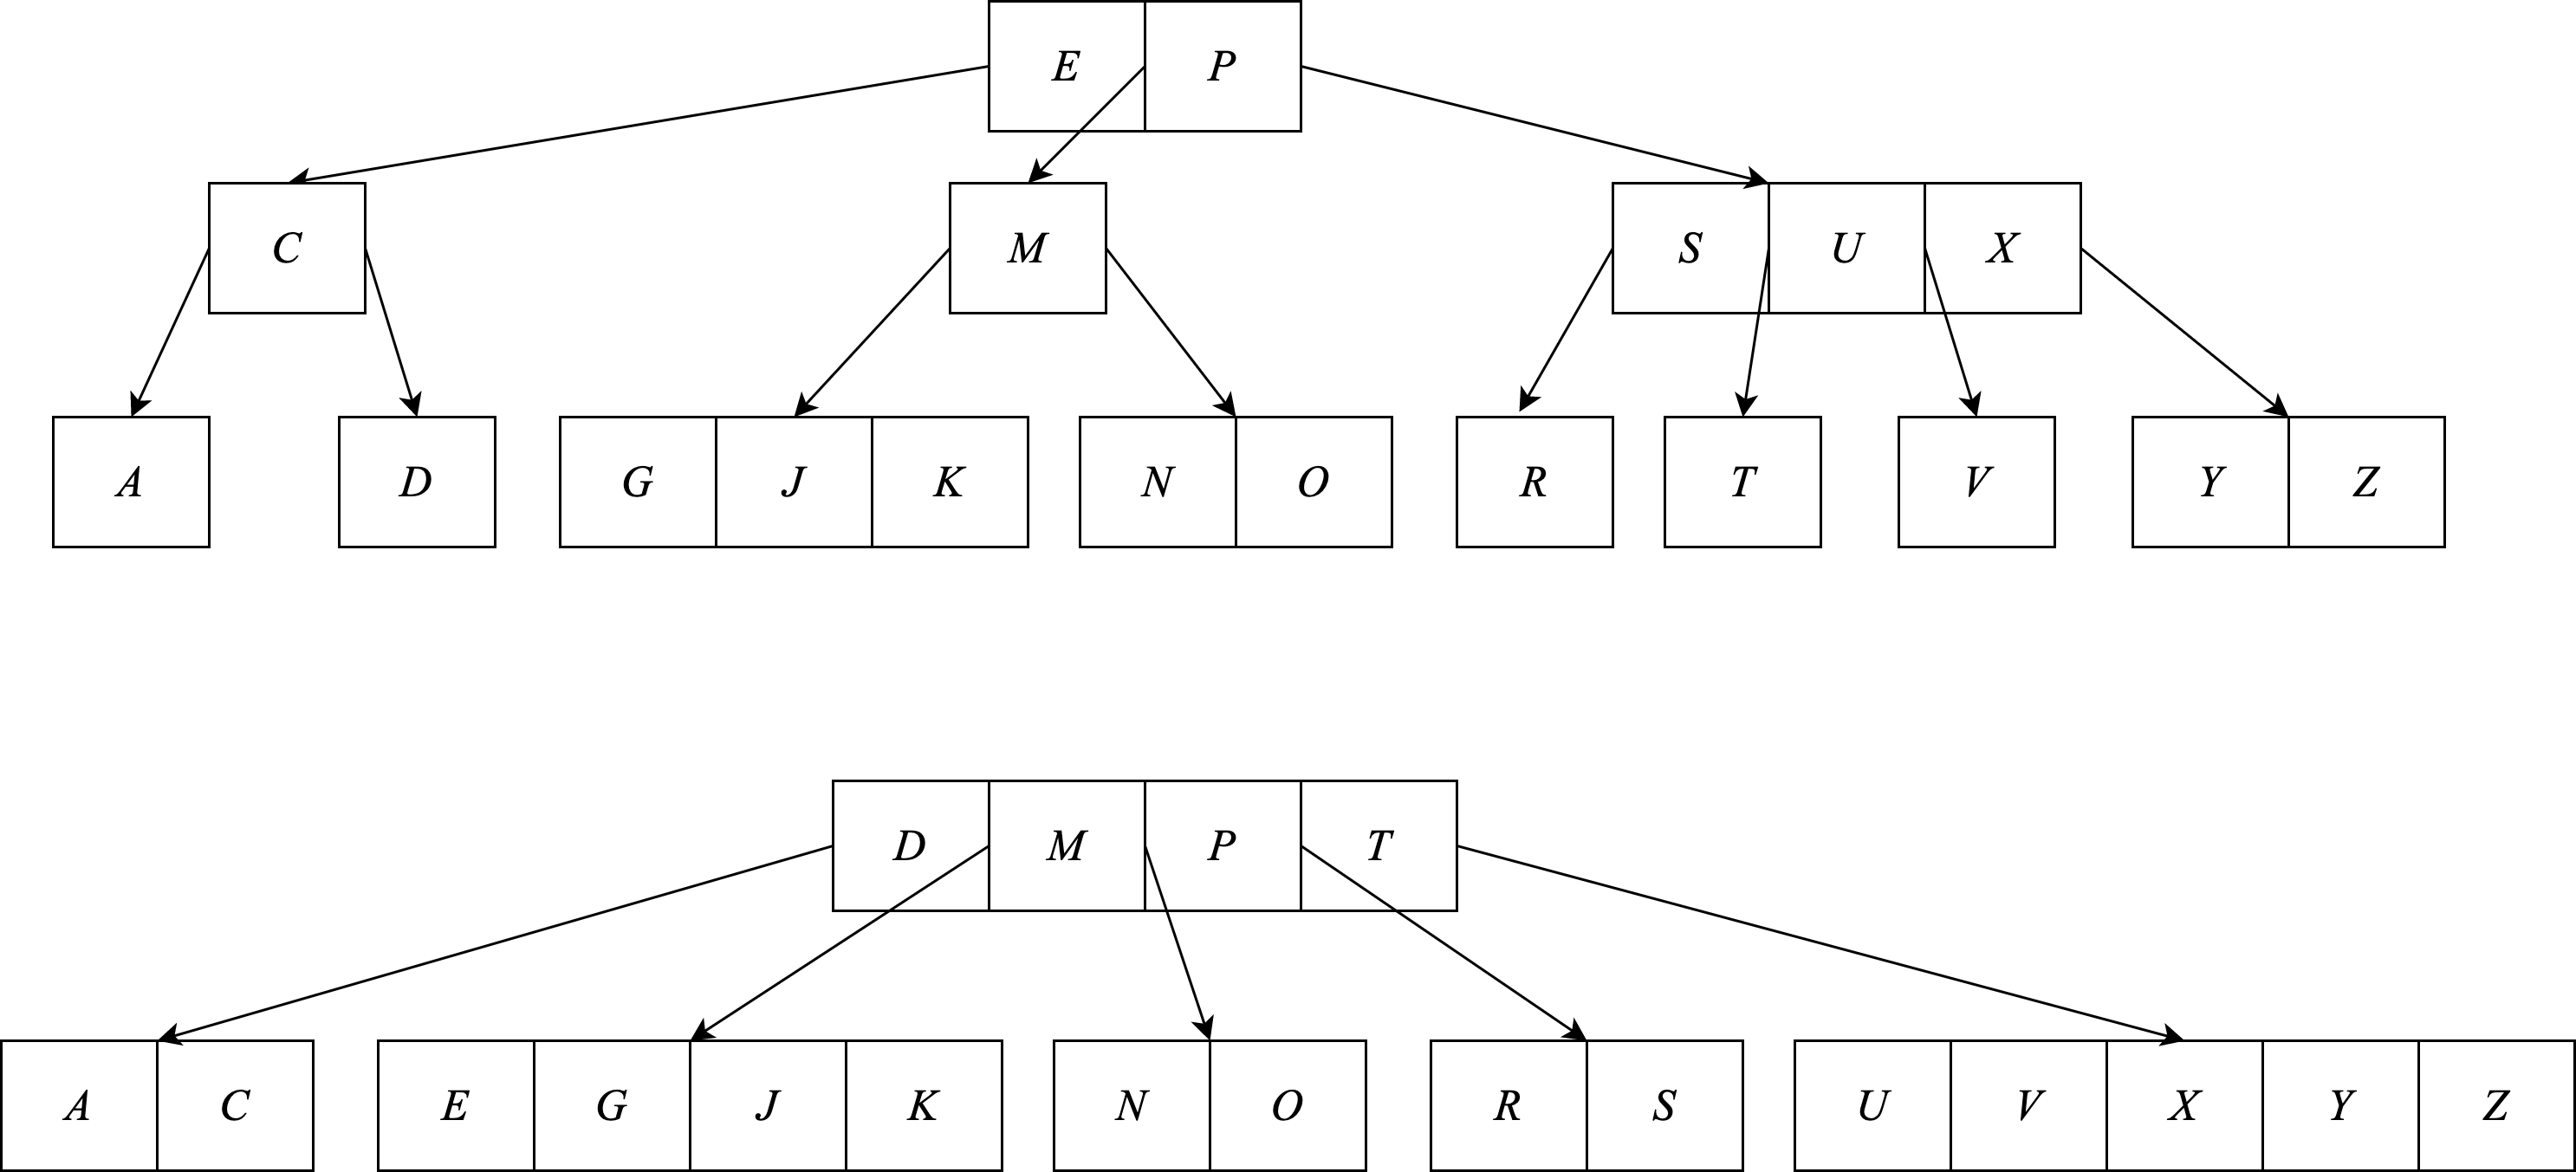
\includegraphics[scale=0.5]{img/btree-split-insert-example}
  \caption{依次插入``GMPXACDEJKNORSTUVYZ''。上:$d = 2$(2-3-4树),下:$d = 3$}
  \label{fig:btree-insert}
\end{figure}

\subsection{列表对}

用列表存储元素时,我们需要从第一个元素开始,扫描列表找到插入位置。如果用数组存储,我们可以使用二分查找。可否从节点中的某个位置开始,根据元素的大小向左或向右前进呢?我们可以将B树节点表示为三部分:某棵子分枝$t'$,它的左侧$l$,右侧$r$。其中左右侧都是“元素/子分枝”对$(k_i, t_i)$的列表。特别的,左侧$l$是逆序的。$l$和$r$经由$t'$头对头地连接起来,组成一个如\cref{fig:paired-lists}所示的马蹄形。我们可以用常数时间前后移动。

\begin{figure}[htbp]
  \centering
  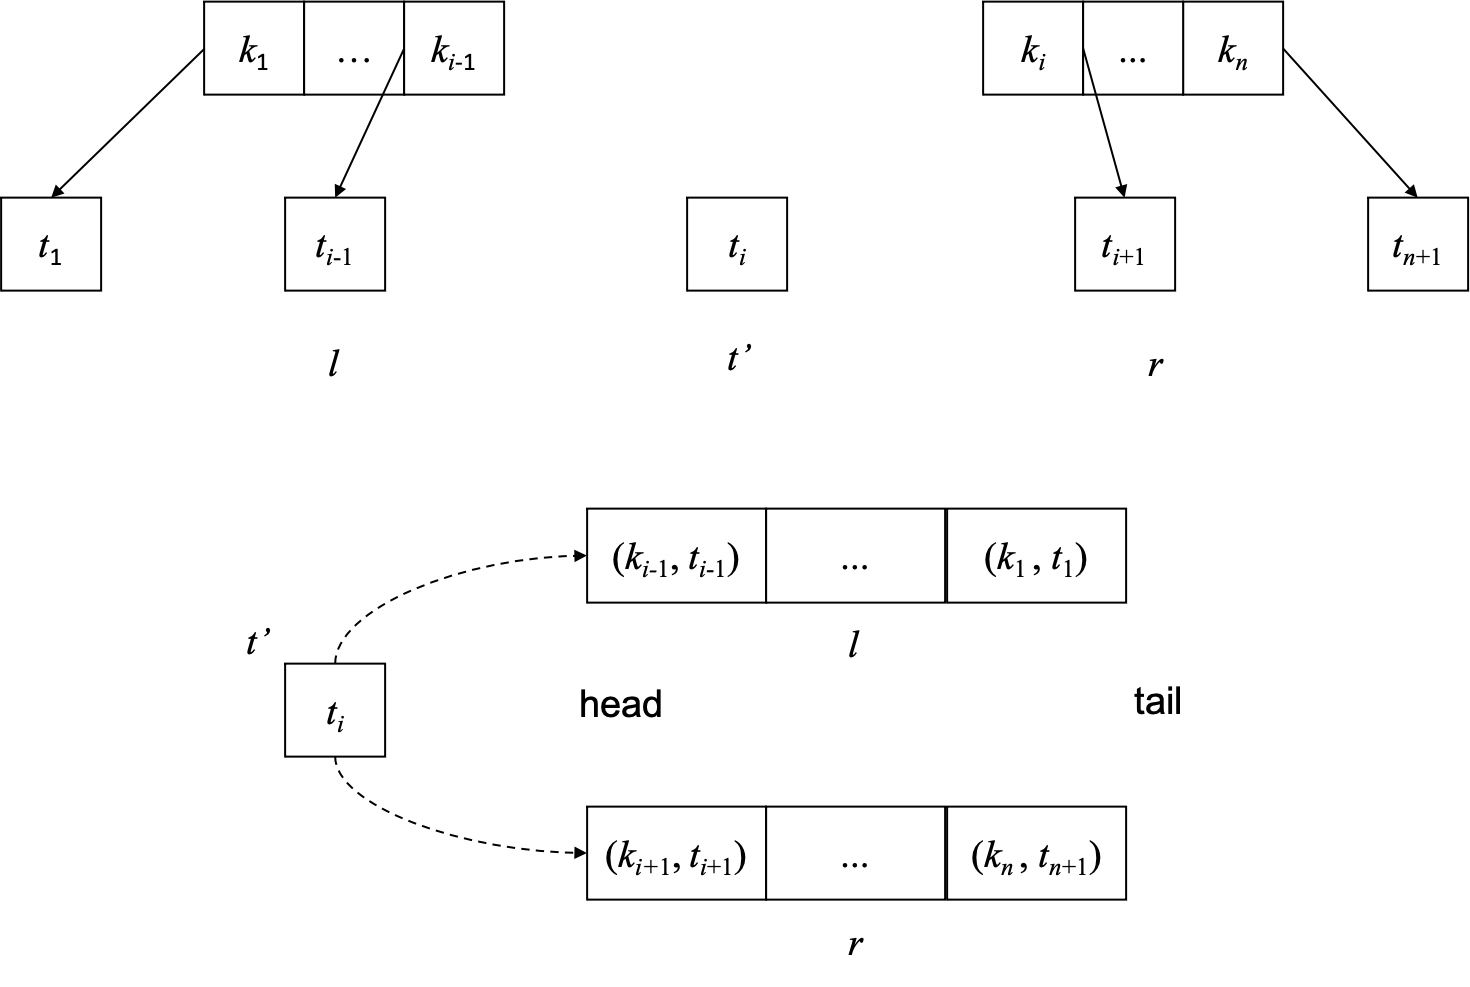
\includegraphics[scale=0.45]{img/paired-lists}
  \caption{将B树表示为某个子分枝和它两侧的一对列表}
  \label{fig:paired-lists}
\end{figure}

下面的例子程序用列表对定义了B树节点。它或者为空,或者包含三部分:左侧逆序的(元素,子分枝)列表,中间的某个子分枝,右侧的(元素、子分枝)列表。我们记非空的节点为$(l, t', r)$。

\begin{Haskell}
data BTree a = Empty
           | BTree [(a, BTree a)] (BTree a) [(a, BTree a)]
\end{Haskell}

向右移动一步时,我们从$r$中取出第一对值$(k, t)$,组成另一对$(k, t')$置于$l$的最前面。然后用$t$替换$t'$。向左移动的步骤与此对称。它们都只需要常数时间。

\be
\begin{array}{lcl}
  step_l\ ((k, t):l, t', r) & = & (l, t, (k, t'):r) \\
  step_r\ (l, t', (k, t):r) & = & ((k, t'):l, t, r) \\
\end{array}
\ee

利用左右移动,我们可以实现划分函数$partition\ p\ t$,根据条件$p$把B树$t$分成左中右三部分:$(l, m, r)$。所有$l$中的分枝和$m$都满足$p$,而$r$中的分枝不满足。定义函数$hd = fst \circ head$,它从列表中取出第一对值$(a, b)$,然后再获取$a$。

\be
\begin{array}{lcl}
  partition\ p\ (\nil, m, r) & = & \begin{cases}
    p(hd(r)): & partition\ p\ (step_r\ t) \\
    otherwise: & (\nil, m, r) \\
  \end{cases} \\
  partition\ p\ (l, m, \nil) & = & \begin{cases}
    (not \circ p)(hd(l)): & partition\ p\ (step_l\ t) \\
    otherwise: & (l, m, \nil) \\
  \end{cases}\\
  partition\ p\ (l, m, r) & = & \begin{cases}
    p(hd(l))\ \text{and}\ (not \circ p)(hd(r)): & (l, m, r) \\
    p(hd(r)): & partition\ p\ (step_r\ t) \\
    (not \circ p)(hd(l)): & partition\ p\ (step_l\ t) \\
  \end{cases}
\end{array}
\ee

例如$partition\ (<k)\ t$将$t$中所有不小于$k$的元素和分枝留在右侧。下面的例子程序实现了$partition$函数:

\begin{Haskell}
partition p t@(BTree [] m r)
  | p (hd r) = partition p (stepR t)
  | otherwise = ([], m, r)
partition p t@(BTree l m [])
  | (not . p) (hd l) = partition p (stepL t)
  | otherwise = (l, m, [])
partition p t@(BTree l m r)
  | p (hd l) && (not . p) (hd r) = (l, m, r)
  | p (hd r) = partition p (stepR t)
  | (not . p) (hd l) = partition p (stepL t)
\end{Haskell}

我们也可以利用$step_l/step_r$把含有过多元素的节点在位置$d$拆分。令$n = |l|$表示左侧的“元素/子分枝”数量。$f^n(x)$表示对变量$x$重复应用函数$f$共$n$次。

\be
split\ d\ t = \begin{cases}
  n < d: & sp(step_r^{d - n}(t)) \\
  n > d: & sp(step_r^{n - d}(t)) \\
  otherwise: & sp(t) \\
  \end{cases}
\ee

其中$sp$进行如下的分拆:

\be
sp\ (l, t, (k, t'):r) = ((l, t, \nil), k, (\nil, t', r))
\ee

利用$partition$和$split$,对于列表对表示的B树,我们可以定义出插入算法。首先我们需要修改B树含有过多、过少元素的判断:

\be
\begin{array}{ll}
  full\ d\ \nil & = False \\
  full\ d\ (l, t', r) & = |l| + |r| > 2d - 1 \\
\end{array}
\ee
和
\be
\begin{array}{ll}
  low\  d\ \nil & = False \\
  low\  d\ (l, t', r) & = |l| + |r| < d - 1 \\
\end{array}
\ee

向度数为$d$的B树$t$插入元素$x$时,我们首先递归地插入,然后再修复元素过多的问题:

\be
insert\ x\ (d, t) = fix\ (d, ins\ t)
\ee

如果根节点含有过多元素,函数$fix$在位置$d$将其分拆:

\be
fix\ (d, t) = \begin{cases}
  full\ d\ t: & (d, (\nil, t_1, [(k, t_2)]\ \text{其中}\ (t_1, k, t_2) = split\ d\ t \\
  otherwise: & (d, t)
  \end{cases}
\ee

函数$ins$需要处理$t = \nil$和$t \neq \nil$两种情况。对于空树,我们新建一个单独的叶子节点;否则调用$(l, t', r) = partition\ (< x)\ t$定位到递归插入的位置:

\be
\begin{array}{lcl}
  ins\ \nil & = & (\nil, \nil, [(x, \nil)]) \\
  ins\ t & = & \begin{cases}
    t' = \nil: & balance\ d\ l\ \nil\ ((x, \nil):r) \\
    t' \neq \nil: & balance\ d\ l\ (ins\ t')\ r \\
  \end{cases}
\end{array}
\ee

函数$balance$检查子分枝$t$是否包含过多元素并进行分拆。

\be
balance\ d\ l\ t\ r = \begin{cases}
  full\ d\ t: & fixFull \\
  otherwise: & (l, t, r)
  \end{cases}
\ee

其中$fixFull = (l, t_1, ((k, t_2):r)$,$(t_1, k, t_2) = split\ d\ t$。下面的例子程序实现了插入算法:

\begin{Haskell}
insert x (d, t) = fixRoot (d, ins t) where
  ins Empty = BTree [] Empty [(x, Empty)]
  ins t = let (l, t', r) = partition (< x) t in
    case t' of
      Empty -> balance d l Empty ((x, Empty):r)
      _     -> balance d l (ins t') r

fixRoot (d, t) | full d t = let (t1, k, t2) = split d t in
                   (d, BTree [] t1 [(k, t2)])
               | otherwise = (d, t)

balance d l t r | full d t = fixFull
                | otherwise = BTree l t r
  where
    fixFull = let (t1, k, t2) = split d t in BTree l t1 ((k, t2):r)

split d t@(BTree l _ _) | n < d = sp $ iterate stepR t !! (d - n)
                        | n > d = sp $ iterate stepL t !! (n - d)
                        | otherwise = sp t
  where
    n = length l
    sp (BTree l t ((k, t'):r)) = (BTree l t [], k, BTree [] t' r)
\end{Haskell}

\begin{Exercise}\label{ex:btree-insert}
\Question{我们是否可以用$\leq$使得B树含有重复元素?}\label{ex:btree-leq}
\Question{使用循环消除“先分拆再插入”算法中的递归。}\label{ex:btree-loop-insert}
\Question{我们使用线性查找获得元素插入的位置。请使用二分查找对命令式实现进行改进。算法复杂度会提升么?}\label{ex:btree-binary-search}
\end{Exercise}

\begin{Answer}[ref = {ex:btree-insert}]
\Question{我们是否可以用$\leq$使得B树含有重复元素?

可以用$\leq$使B树包含重复元素:所有左侧元素小于等于$x$,而$x$小于等于所有右侧元素。但在查找、删除时需要额外处理重复元素。一般我们限制B树中的键唯一,而一个键可以对应多个值($k \mapsto [v_1, v_2, ...]$),称为多值映射(multimap)。
}

\Question{使用循环消除“先分拆再插入”算法中的递归。

\begin{Bourbaki}
BTree<K, deg> insertNonfull(BTree<K, deg> tr, K key) {
    var root = t
    while not is_leaf(t) {
        Int i = length(t.keys)
        while i > 0 and key < t.keys[i-1] {
            i = i - 1
        }
        if full(d, t.subTrees[i]) {
            split(d, t, i)
            if key > t.keys[i] then i = i + 1
        }
        t = t.subTrees[i]
    }
    orderedInsert(t.keys, key)
    return root
\end{Bourbaki}
}

\Question{我们使用线性查找获得元素插入的位置。请使用二分查找对命令式实现进行改进。算法复杂度会提升么?

\begin{Bourbaki}
void orderedInsert([K] xs, K x) {
    append(xs, x)
    Int p = binarySearch(xs, x)
    for Int i = length(lst), i > p, i = i - 1 {
        xs[i] = xs[i-1]
    }
}

Int binarySearch([K] xs, K x) {
    Int l = 0, u = length(xs)
    while l < u {
        Int m = (l + u) / 2
        if xs[m] == x {
            return m
        } else if xs[m] < x {
            l = m + 1
        } else {
            u = m
        }
    }
    return l
}
\end{Bourbaki}

复杂度仍然是线性时间的。尽管二分查找需要$O(\lg n)$时间,但是插入需要$O(n)$时间移动数组以获取空位。
}
\end{Answer}

\section{查找}
\index{B树!查找}

我们可以将二叉搜索树的查找算法扩展到含有多个分枝的B树。二叉树查找只有左右两个方向,但B树有多个方向。考虑在B树$t = (ks, ts)$中查找元素$k$,如果$t$是叶子节点($ts$为空),则问题简化为列表查找;否则,我们用$k$将树$t$划分为三部分:$l = (ks_l, ts_l)$、$t'$、$r = (ks_r, ts_r)$,其中$l$和子分枝$t'$中的所有元素都小于$k$,而$r$中的所有元素大于等于$k$。如果$r$中的第一个元素$ks_r$等于$k$,我们就找到了结果;否则我们递归地在子分枝$t'$中查找。

\be
\begin{array}{lcl}
  lookup\ k\ (ks, \nil) & = & \begin{cases}
    k \in ks: & \textit{Just}\ (ks, \nil) \\
    otherwise: & \textit{Nothing}
  \end{cases} \\
  lookup\ k\ (ks, ts) & = & \begin{cases}
    \textit{Just}\ k = \textit{safeHd}\ ks_r: & \textit{Just}\ (ks, ts) \\
    otherwise: & lookup\ k\ t' \\
  \end{cases}\\
\end{array}
\ee

其中$((ks_l, ts_l), t', (ks_r, ts_r)) = partition\ k\ t$。函数\textit{safeHd}定义为:

\[
\begin{array}{lcl}
  \textit{safeHd}\ [] & = & \textit{Nothing} \\
  \textit{safeHd}\ (x:xs) & = & \textit{Just}\ x \\
\end{array}
\]

下面的例子程序\footnote{\texttt{safeHd}在某些程序库中以\texttt{listToMaybe}提供}实现了查找算法。

\begin{Haskell}
lookup k t@(BTree ks []) = if k `elem` ks then Just t else Nothing
lookup k t = if (Just k) == safeHd ks then Just t
             else lookup k t'  where
  (_, t', (ks, _)) = partition k t
\end{Haskell}

对于列表对实现,思路是类似的。如果树不为空,我们用条件“$< k$”进行划分。然后检查右侧部分的第一个元素是否等于$k$,否则再递归地进行查找:

\be
\begin{array}{lcl}
  lookup\ k\ \nil & = & \textit{Nothing} \\
  lookup\ k\ t & = & \begin{cases}
    \textit{Just}\ k = \textit{safeFst}\ (\textit{safeHd}\ r): & \textit{Just}\ (l, t', r) \\
    otherwise: & lookup\ k\ t' \\
    \end{cases}
\end{array}
\ee

其中$(l, t', r) = partition\ (< k)\ t$是对非空树的划分。\textit{safeFst}将函数\textit{fst}应用到“Maybe”的值上,下面的例子程序使用了\textit{fmap}来实现:

\begin{Haskell}
lookup x Empty = Nothing
lookup x t = let (l, t', r) = partition (< x) t in
  if (Just x) == fmap fst (safeHd r) then Just (BTree l t' r)
  else lookup x t'
\end{Haskell}

对于命令式实现,我们从根节点$r$开始,找到位置$i$使得$k_i(r) \leq k < k_{i+1}(r)$。如果$k_i(r) = k$,则返回节点$r$和索引$i$组成的值对;否则,我们继续在子分枝$t_i(r)$中继续查找。如果$r$是叶子节点,并且$k$不在其中,则返回空结果。

\begin{algorithmic}[1]
\Function{Look-Up}{$r, k$}
  \Loop
    \State $i \gets 1, n \gets |K(r)|$
    \While{$i \leq n$ and $k > k_i(r)$}
      \State $i \gets i + 1$
    \EndWhile
    \If{$i \leq n$ and $k = k_i(r)$}
      \State \Return $(r, i)$
    \EndIf
    \If{$r$ is leaf}
      \State \Return Nothing \Comment{$k$不存在}
    \Else
      \State $r \gets t_i(r)$ \Comment{继续查找第$i$棵分枝}
    \EndIf
  \EndLoop
\EndFunction
\end{algorithmic}

\begin{Exercise}
  \Question{使用二分查找改进命令式查找算法。}
\end{Exercise}

\section{删除}
\index{B树!删除}

删除元素后,节点可能因为元素不足无法满足B树的要求。除根节点外,元素数不能小于$d - 1$,其中$d$是最小度数。对称于插入算法,我们也有两种解法:先删除再修复、先合并再删除。

\subsection{先删除再修复}

我们首先扩展二叉搜索树的删除算法到多个分枝,然后再修复B树的平衡性。算法包含两步:

\be
delete\ x\ (d, t) = fix (d, del\ x\ t)
\ee

其中函数$del$是对多分枝扩展的删除操作。如果$t$是叶子节点,我们从节点元素中删除$x$;否则,我们用$x$将树划分为三部分:$(l, t', r)$。其中$l$和$t'$的所有元素小于$x$,而$r$中的其余元素大于等于($\geq$)$x$。如果$r$不为空,我们取出其中的第一个元素$k_i$,若它等于$x$(即$k_i = x$),我们接下来用子分枝$t'$中的最大元素$k'$(即$k' = max(t')$)取代$k_i$。然后递归地从$t'$中删除$k'$,如\cref{fig:btree-del}所示。否则($r$为空或$k_i \neq x$),我们递归地从$t'$中删除$x$。

\begin{figure}[htbp]
  \centering
  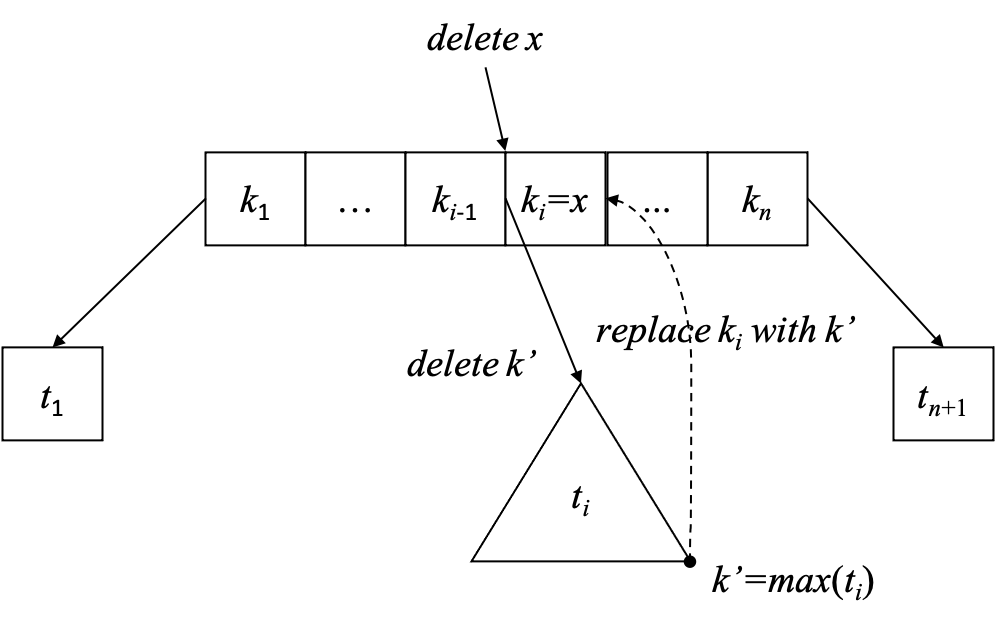
\includegraphics[scale=0.45]{img/btree-del}
  \caption{用$k' = max(t')$替换$k_i$,然后递归地从$t'$删除$k'$}
  \label{fig:btree-del}
\end{figure}

\be
\begin{array}{lcl}
del\ x\ (ks, \nil) & = & (delete_l\ x\ ks, \nil) \\
del\ x\ t & = & \begin{cases}
  \textit{Just}\ x = \textit{safeHd}\ ks': & balance\ d\ l\ (del\ k'\ t')\ (k':(tail\ ks'), ts') \\
  otherwise: & balance\ d\ l\ (del\ x\ t')\ (ks', ts') \\
  \end{cases}
\end{array}
\ee

其中$(l, t', (ks', ts')) = partition\ x\ t$,是用$x$进行划分的三部分。我们可以进一步从$t'$中获得最大元素$k'$。函数$max$定义如下:

\be
\begin{array}{lcl}
  max\ (ks, \nil) & = & last\ ks \\
  max\ (ks, ts) & = & max\ (last\ ts) \\
\end{array}
\ee

函数$last$返回列表中的最后一个元素(第一章\cref{eq:list-last})。$delete_l$是第一章\cref{eq:list-delete}中定义的列表删除函数。$tail$将列表中的第一个元素去掉,并返回剩下的元素\cref{eq:list-head-tail}。我们还需要修改此前在插入算法中定义的$balance$函数。如果节点中的元素太少,就进行合并。

\be
balance\ d\ (ks_l, ts_l)\ t\ (ks_r, ts_r) = \begin{cases}
  full\ d\ t: fix_f \\
  low\ d\ t: fix_l \\
  otherwise: (ks_l \doubleplus ks_r, ts_l \doubleplus [t] \doubleplus ts_r)
  \end{cases}
\ee

如果$t$中的元素不足($< d - 1$),我们调用$fix_l$与左侧$(ks_l, ts_l)$或右侧$(ks_r, ts_r)$合并(选择一个不为空的)。以左侧为例:我们从$ks_l$、$ts_l$中取出最后的元素$k_m$、$t_m$。然后调用$unsplit$(\autoref{eq:btree-unsplit})和$t$合并:$unsplit\ t_m\ k_m\ t$。构造一个含有更多元素的新分枝。最后,我们再次调用$balance$函数构造最终的B树。

\be
fix_l = \begin{cases}
  ks_l \neq \nil: & balance\ d\ (init\ ks_l, init\ ts_l)\ (unsplit\ t_m\ k_m\ t)\ (ks_r, ts_r) \\
  ks_r \neq \nil: & balance\ d\ (ks_l, ts_l)\ (unsplit\ t\ k_1\ t_1)\ (tail\ ks_r, tail\ ts_r) \\
  otherwise: & t
  \end{cases}
\ee

上式最后一种情况中$ks_l = ks_r = \nil$,两侧都为空。这是一棵只有一个叶子的树,无需进一步修复。$k_1$和$t_1$分别是$ks_r$和$ts_r$中的第一个元素。最后我们修改此前插入算法中定义的$fix$函数,加入删除的处理逻辑:

\be
\begin{array}{lcl}
fix\ (d, (\nil, [t])) & = & (d, t) \\
fix\ (d, t) & = & \begin{cases}
  full\ d\ t : & (d, ([k], [l, r])), \text{其中}\ (l, k, r) = split\ d\ t \\
  otherwise  : & (d, t)
\end{cases}
\end{array}
\ee

上式中,我们在最前面加入一条:如果删除后,根节点只包含一棵子树,我们可以缩减高度,将此唯一的子树作为新的根。下面的例子程序实现了删除算法。

\begin{Haskell}
delete x (d, t) = fixRoot (d, del x t) where
    del x (BTree ks []) = BTree (List.delete x ks) []
    del x t = if (Just x) == safeHd ks' then
                let k' = max t' in
                   balance d l (del k' t') (k':(tail ks'), ts')
              else balance d l (del x t') r
      where
        (l, t', r@(ks', ts')) = partition x t

fixRoot (d, BTree [] [t]) = (d, t)
fixRoot (d, t) | full d t  = let (t1, k, t2) = split d t in
                               (d, BTree [k] [t1, t2])
               | otherwise = (d, t)

balance d (ks1, ts1) t (ks2, ts2)
    | full d t  = fixFull
    | low  d t  = fixLow
    | otherwise = BTree (ks1 ++ ks2) (ts1 ++ [t] ++ ts2)
  where
    fixFull = let (t1, k, t2) = split d t in
                BTree (ks1 ++ [k] ++ ks2) (ts1 ++ [t1, t2] ++ ts2)
    fixLow | not $ null ks1 = balance d (init ks1, init ts1)
                                      (unsplit (last ts1) (last ks1) t)
                                      (ks2, ts2)
           | not $ null ks2 = balance d (ks1, ts1)
                                      (unsplit t (head ks2) (head ts2))
                                      (tail ks2, tail ts2)
           | otherwise = t
\end{Haskell}

我们将列表对B树的删除算法留作练习。\cref{fig:btree-del-before}、\cref{fig:btree-del-CJ}、\cref{fig:btree-del-KN}描述了删除的例子。

\begin{figure}[htbp]
  \centering
  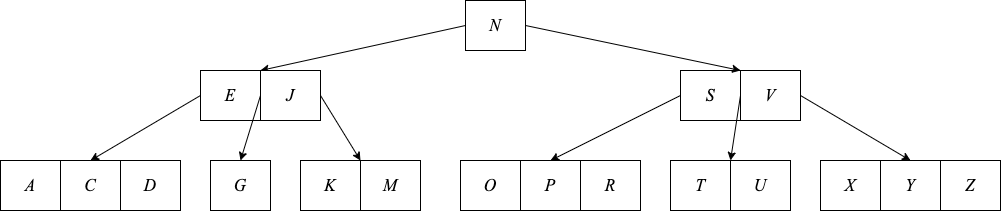
\includegraphics[scale=0.33]{img/btree-del-before}
  \caption{删除前}
  \label{fig:btree-del-before}
\end{figure}

\begin{figure}[htbp]
  \centering
  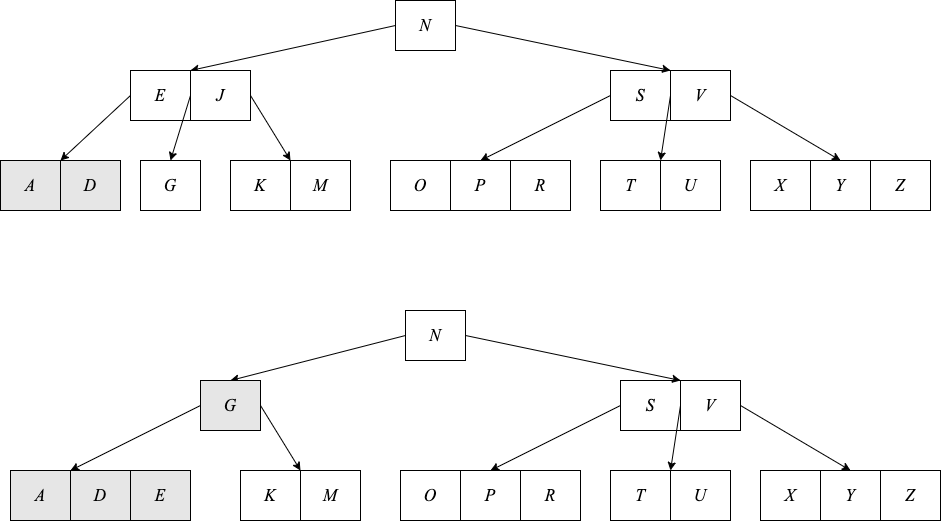
\includegraphics[scale=0.33]{img/btree-del-CJ}
  \caption{删除`C',然后删除`J'}
  \label{fig:btree-del-CJ}
\end{figure}

\begin{figure}[htbp]
  \centering
  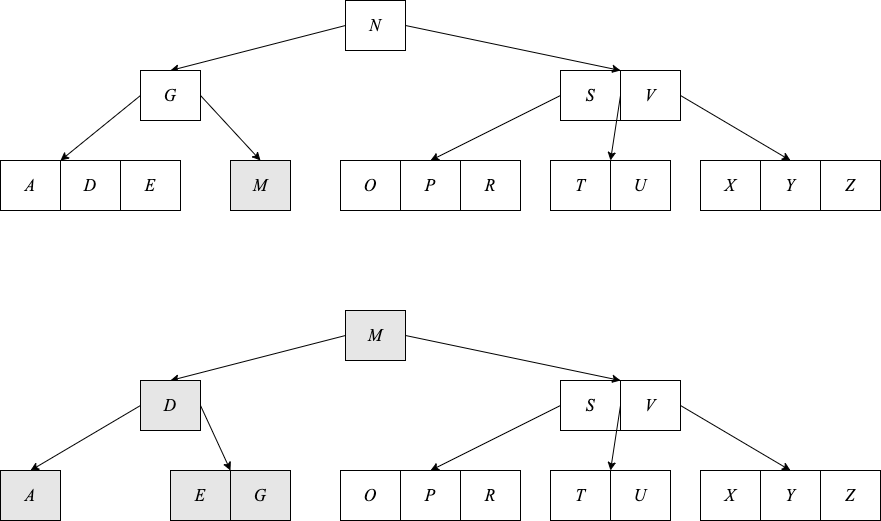
\includegraphics[scale=0.33]{img/btree-del-KN}
  \caption{删除`K',然后删除`N'}
  \label{fig:btree-del-KN}
\end{figure}

\subsection{先合并再删除}

另一种方法是先把元素不足的节点合并,然后再删除。考虑从树$t$中删除元素$x$。我们先从最简单的情况入手。

\textbf{情况1}:如果$x$存在于$t$的元素中,并且$t$是叶子节点。我们可以直接将$t$中的$x$删除。如果$t$是树中的唯一节点(根),则无需进一步修复。

\textbf{情况2}:如果$x$存在于$t$的元素中,但$t$不是叶子节点。则存在三种子情况:

\textbf{情况2a}:如\cref{fig:btree-del}所示,令$k_i = x$的前驱元素为$k'$,其中$k' = max(t_i)$。如果$t_i$含有足够的元素($\geq d$),我们用$k'$替换$k_i$,然后递归地从$t_i$中删除$k'$。

\textbf{情况2b}:如果$t_i$中的元素不足,但是子分枝$t_{i+1}$含有足够的元素($\geq d$),对称地,我们用后继元素$k'' = min(t_{i+1})$替换$k_i$,然后递归地从$t_{i+1}$中删除$k''$。如\cref{fig:btree-del-case2b}所示。

\begin{figure}[htbp]
  \centering
  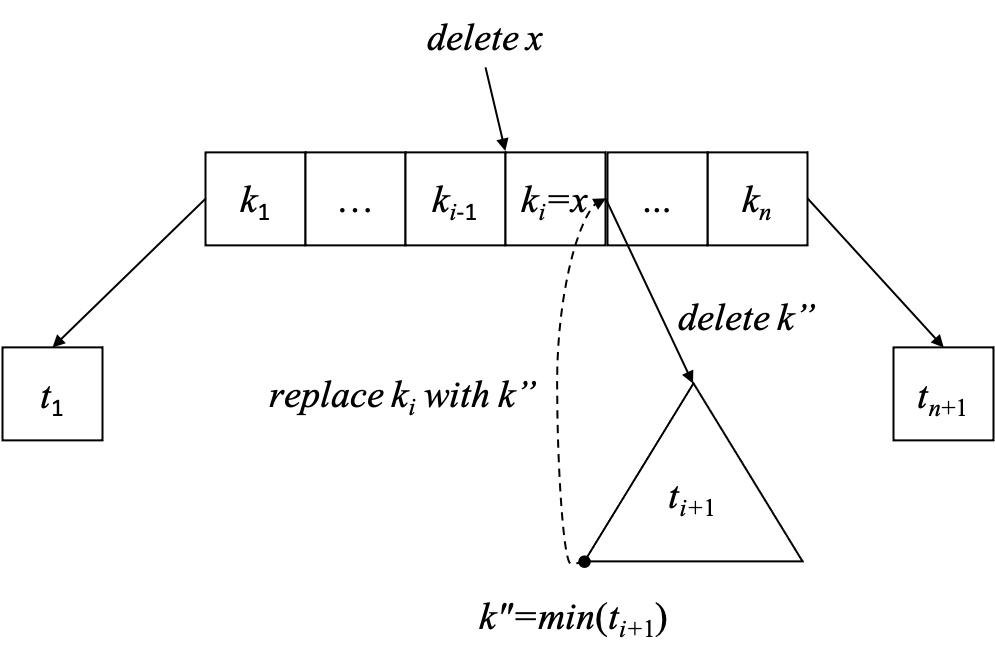
\includegraphics[scale=0.5]{img/btree-del-case2b}
  \caption{用$k'' = min(t_{i+1})$替换$k_i$,然后递归地从$t_{i+1}$中删除$k''$}
  \label{fig:btree-del-case2b}
\end{figure}

\textbf{情况2c}:如果$t_i$和$t_{i+1}$的元素都不足($|t_i| = |t_{i+1}| = d - 1$),我们将$t_i$、$x$、$t_{i+1}$合并成一个新节点。它含有$2d - 1$个元素,可以安全地从中删除。如\cref{fig:btree-del-merge}所示。

\begin{figure}[htbp]
  \centering
  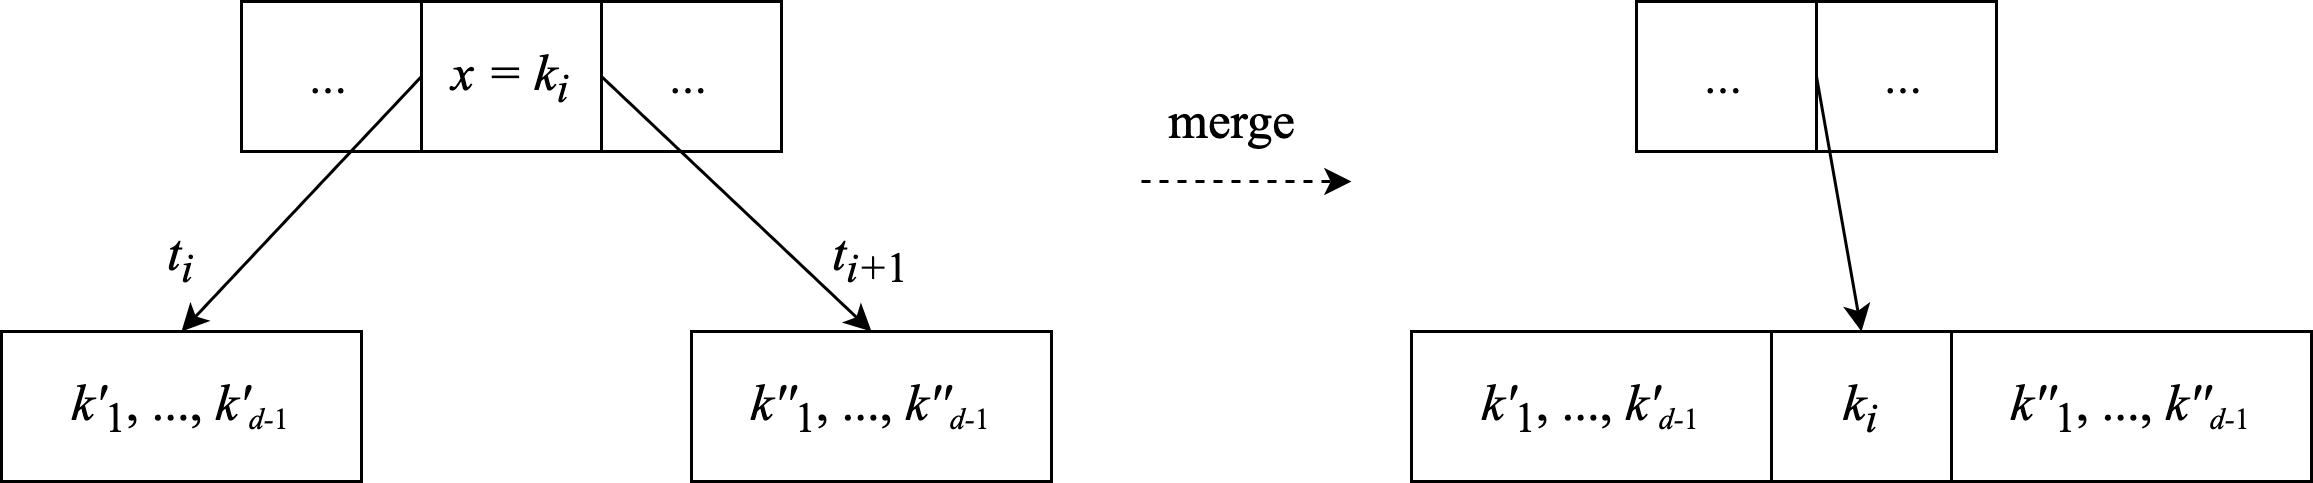
\includegraphics[scale=0.65]{img/btree-del-merge}
  \caption{先合并再删除}
  \label{fig:btree-del-merge}
\end{figure}

合并过程会将元素$k_i$推入子树。如果$t$因此变空(不再含有元素),说明$k_i$是$t$中的唯一元素,并且$t_i$、$t_{i+1}$是仅有的两棵子树。我们可以将树的高度缩减,如\cref{fig:btree-del-shrink}所示。

\begin{figure}[htbp]
  \centering
  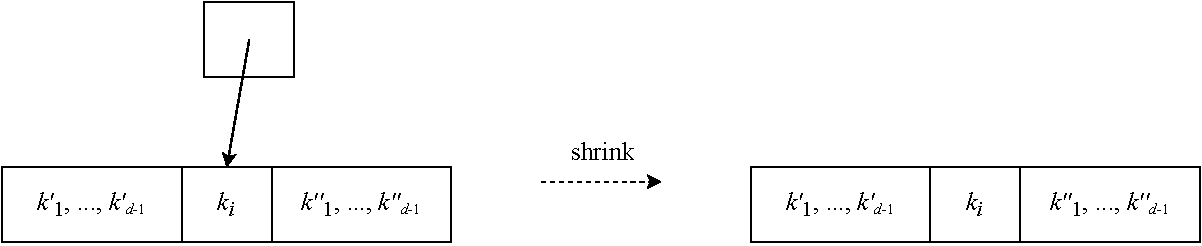
\includegraphics[scale=0.65]{img/btree-del-shrink}
  \caption{缩减高度}
  \label{fig:btree-del-shrink}
\end{figure}

\textbf{情况3}:如果$t$的元素中不包含$x$,我们需要递归地在某个子分枝$t_i$中删除$x$。如果$t_i$中的元素不足,我们需要处理两种子情况:

\textbf{情况3a}:如果$t_i$的两个相邻节点$t_{i-1}$、$t_{i+1}$中的任何一个含有足够的元素($\geq d$),我们将$t$中的一个元素移到$t_i$,然后将相邻节点中的一个元素向上移入$t$,将相应的子分枝移入$t_i$。如\cref{fig:btree-del-borrow}所示,$t_i$获得一个元素。接下来递归地从$t_i$中删除$x$。

\begin{figure}[htbp]
  \centering
  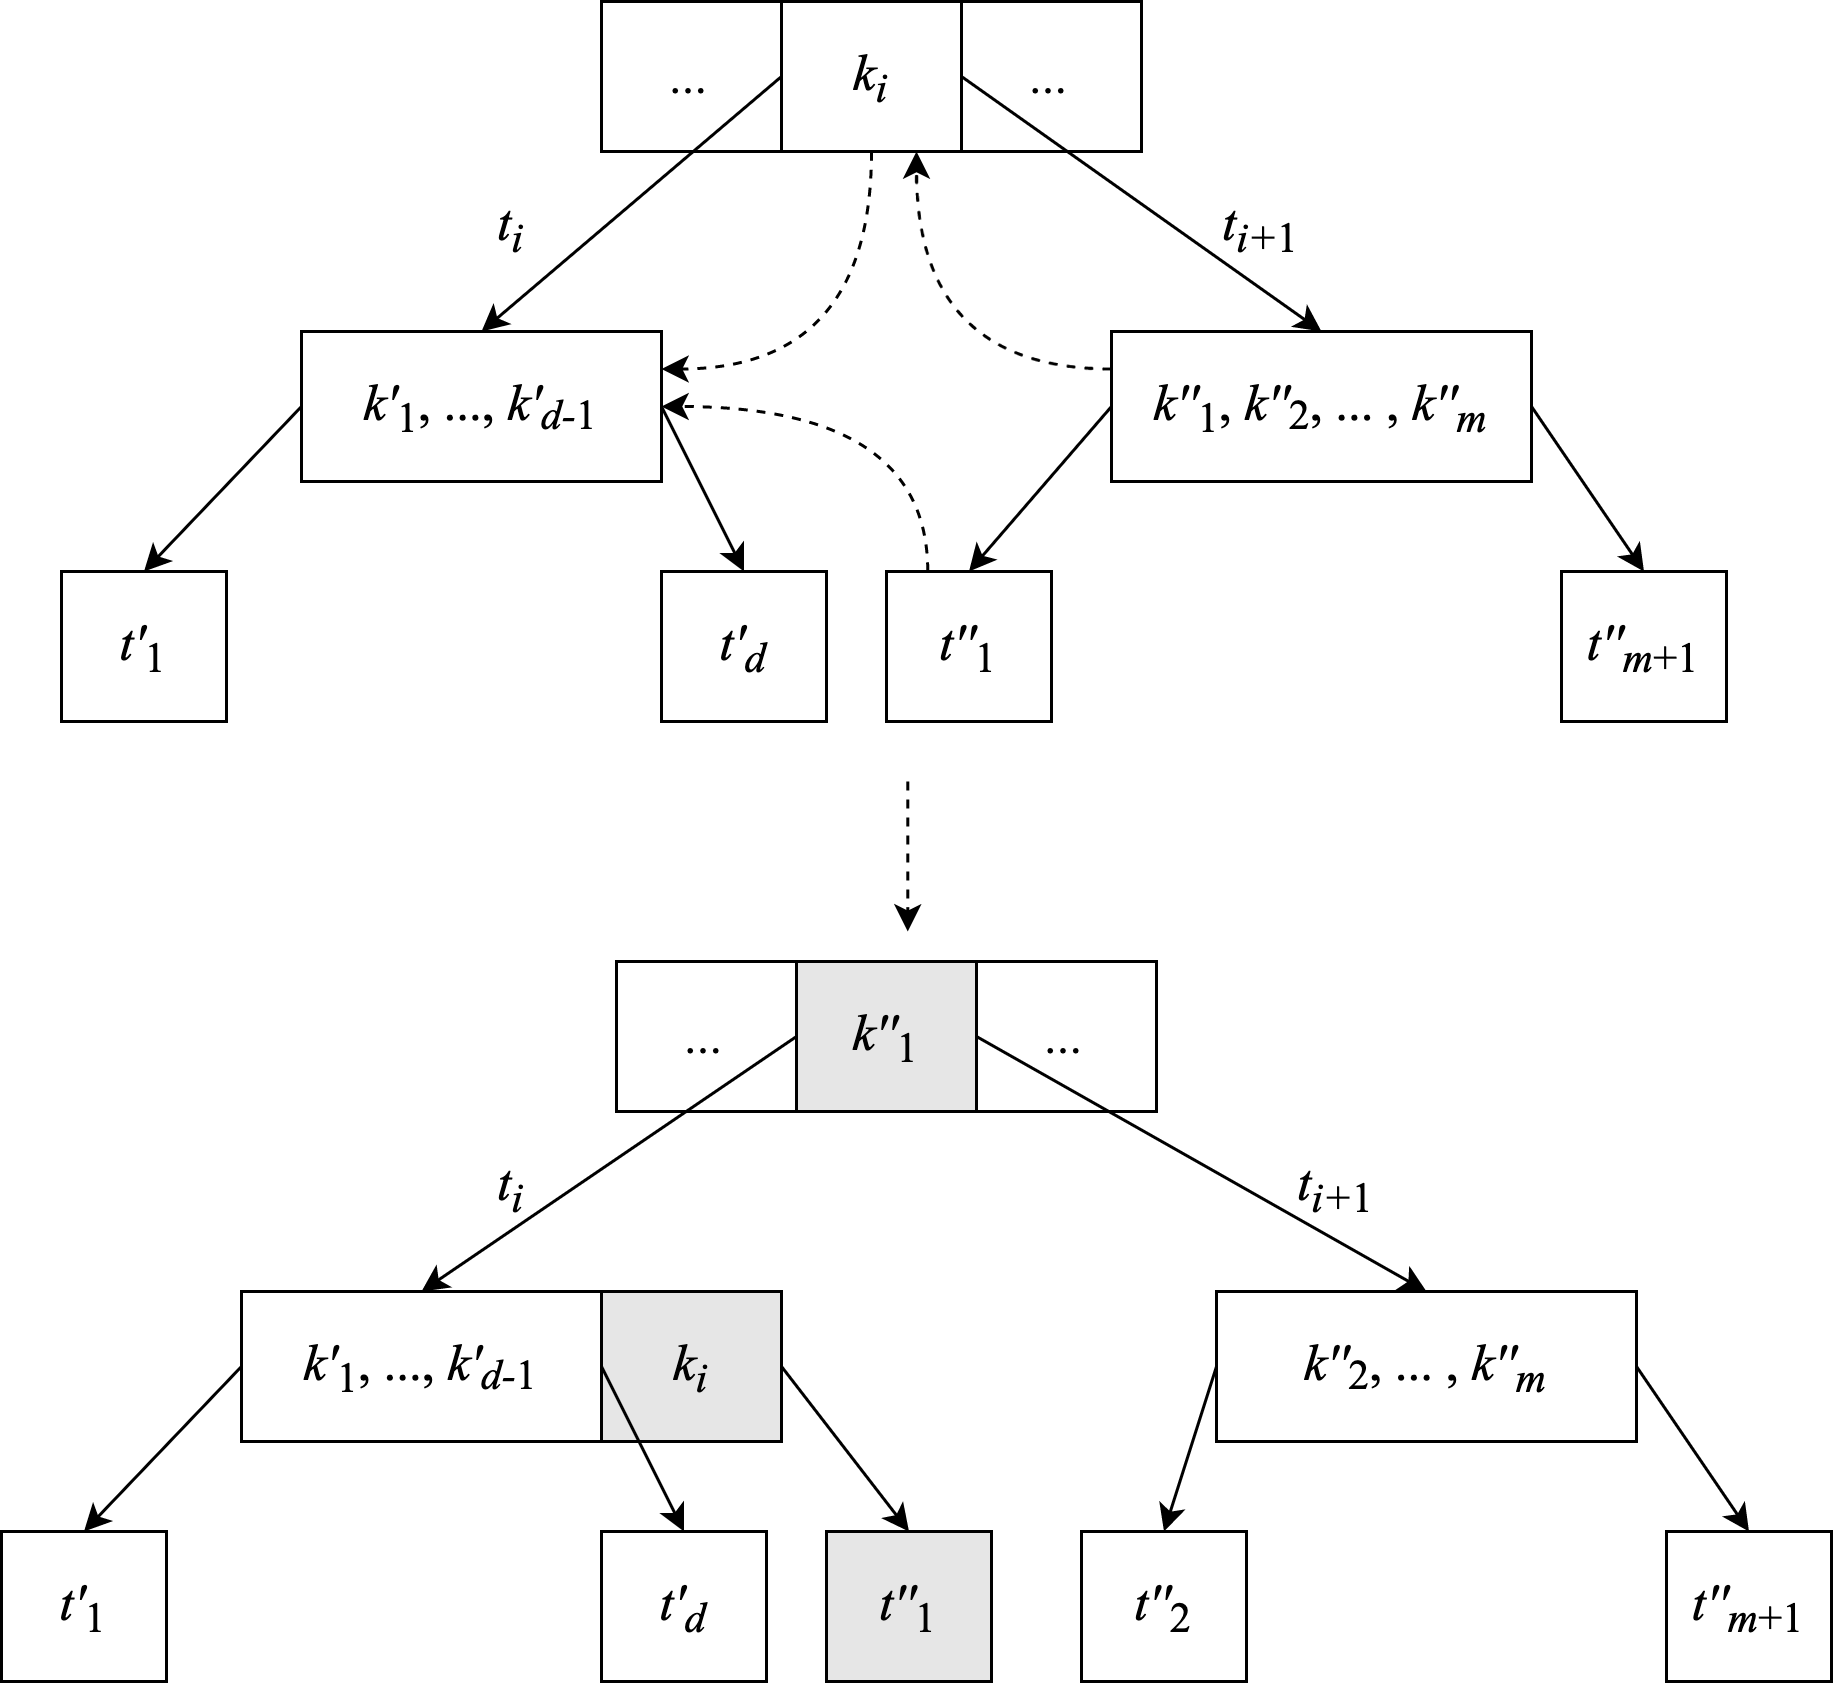
\includegraphics[scale=0.65]{img/btree-del-borrow}
  \caption{从右侧移入一个元素}
  \label{fig:btree-del-borrow}
\end{figure}

\textbf{情况3b}:如果两个相邻节点中的元素都不足($|t_{i-1}| = |t_{i+1}| = d - 1$),我们将$t_i$,$t$中的一个元素,和任一相邻节点合并成一个新节点,如\cref{fig:btree-del-merge-subtree}所示。然后从中递归地删除$x$。

\begin{figure}[htbp]
  \centering
  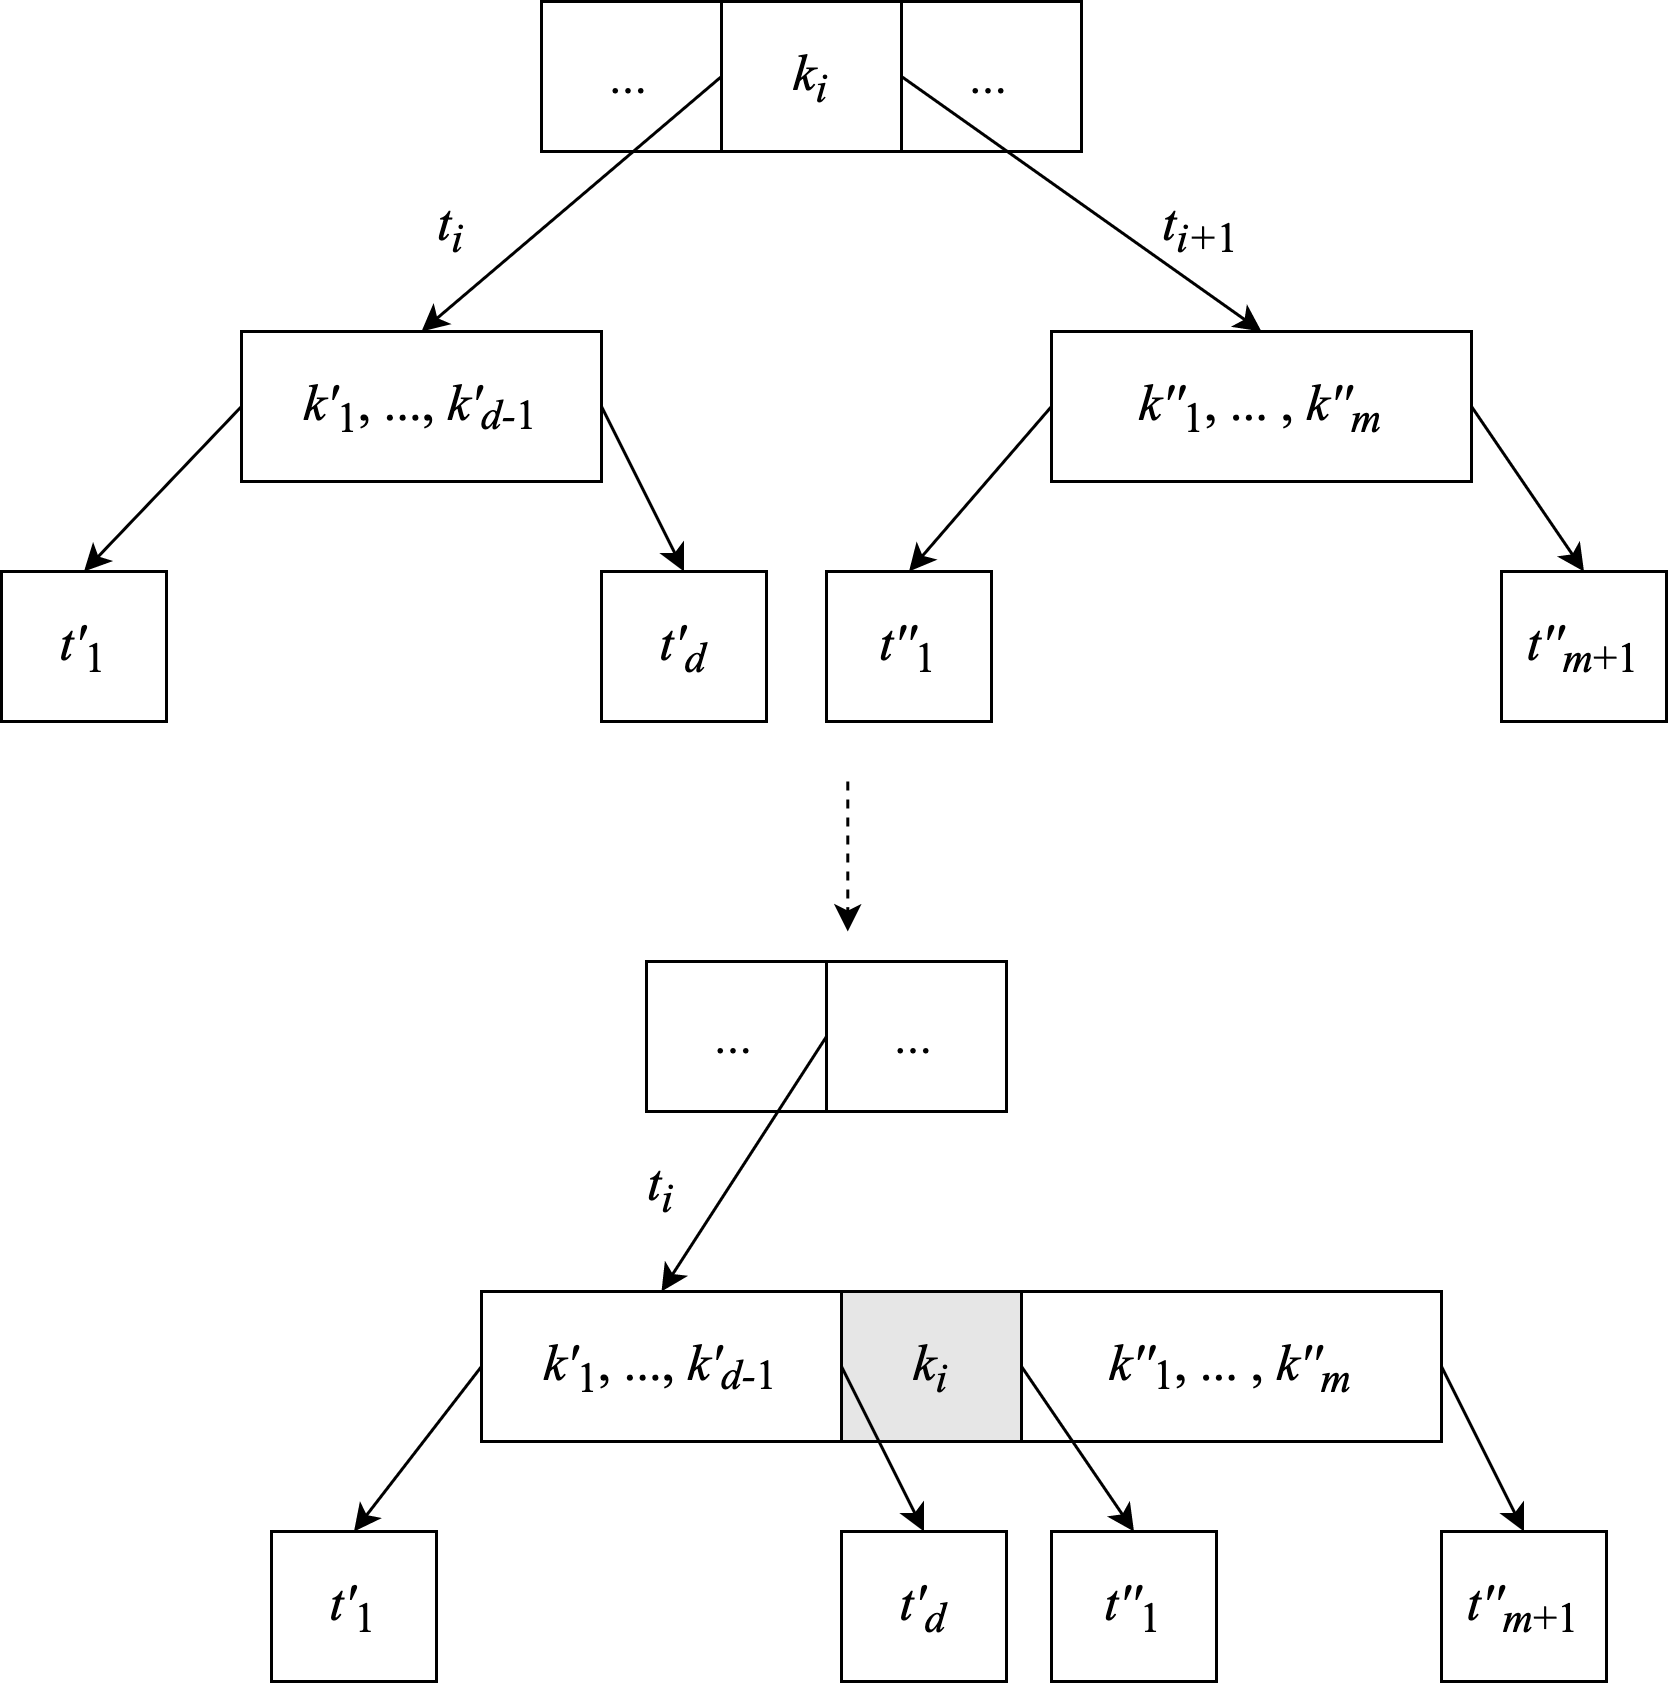
\includegraphics[scale=0.65]{img/btree-del-merge-subtree}
  \caption{合并$t_i$、$k$、$t_{i+1}$}
  \label{fig:btree-del-merge-subtree}
\end{figure}

下面的\textproc{Delete}函数实现了先合并再删除算法:

\begin{algorithmic}[1]
\Function{Delete}{$t, k$}
  \If{$t$ is empty}
    \State \Return $t$
  \EndIf
  \State $i \gets 1$, $n \gets |K(t)|$
  \While{$i \leq n$ and $k > k_i(t)$}
    \State $i \gets i + 1$
  \EndWhile
  \If{$k = k_i(t)$}
    \If{$t$ is leaf} \Comment{情况1}
      \State \Call{Remove}{$K(t), k$}
    \Else \Comment{情况2}
      \If{$|K(t_i(t))| \geq d$} \Comment{情况2a}
        \State $k_i(t) \gets$ \Call{Max}{$t_i(t)$}
        \State \Call{Delete}{$t_i(t), k_i(t)$}
      \ElsIf{$|K(t_{i+1}(t))| \geq d$} \Comment{情况2b}
        \State $k_i(t) \gets$ \Call{Min}{$t_{i+1}(t)$}
        \State \Call{Delete}{$t_{i+1}(t), k_i(t)$}
      \Else \Comment{情况2c}
        \State \Call{Merge-At}{$t, i$}
        \State \Call{Delete}{$t_i(t), k$}
        \If{$K(T)$ is empty}
          \State $t \gets t_i(t)$ \Comment{缩减高度}
        \EndIf
      \EndIf
    \EndIf
    \State \Return $t$
  \EndIf
  \If{$t$ is not leaf}
    \If{$k > k_n(t)$}
      \State $i \gets i + 1$
    \EndIf
    \If{$|K(t_i(t))| < d$}  \Comment{情况3}
      \If{$i > 1$ and $|K(t_{i-1}(t))| \geq d$} \Comment{情况3a:左}
        \State \Call{Insert}{$K(t_i(t)), k_{i-1}(t)$}
        \State $k_{i-1}(t) \gets$ \Call{Pop-Last}{$K(t_{i-1}(t))$}
        \If{$t_i(t)$ is not leaf}
          \State \textproc{Insert}($T(t_i(t))$, \Call{Pop-Back}{$T(t_{i-1}(t))$})
        \EndIf
      \ElsIf{$i \leq n$ and $|K(t_{i+1}(t))| \geq d$} \Comment{情况3a:右}
        \State \Call{Append}{$K(t_i(t)), k_i(t)$}
        \State $k_i(t) \gets$ \Call{Pop-First}{$K(t_{i+1}(t))$}
        \If{$t_i(t)$ is not leaf}
          \State \textproc{Append}($T(t_i(t))$, \Call{Pop-First}{$T(t_{i+1}(t))$})
        \EndIf
      \Else \Comment{情况3b}
        \If{$i = n + 1$}
          \State $i \gets i - 1$
        \EndIf
        \State \Call{Merge-At}{$t, i$}
      \EndIf
    \EndIf
    \State \Call{Delete}{$t_i(t), k$}
    \If{$K(t)$ is empty} \Comment {缩减高度}
      \State $t \gets t_1(t)$
    \EndIf
  \EndIf
  \State \Return $t$
\EndFunction
\end{algorithmic}

其中\textproc{Merge-At}($t, i$)将分枝$t_i(t)$、元素$k_i(t)$、分枝$t_{i+1}(t)$合并成一个新分枝。

\begin{algorithmic}[1]
\Procedure{Merge-At}{$t, i$}
  \State $x \gets t_i(t)$
  \State $y \gets t_{i+1}(t)$
  \State $K(x) \gets K(x) \doubleplus [k_i(t)] \doubleplus K(y)$
  \State $T(x) \gets T(x) \doubleplus T(y)$
  \State \Call{Remove-At}{$K(t), i$}
  \State \Call{Remove-At}{$T(t), i+1$}
\EndProcedure
\end{algorithmic}

\begin{Exercise}
  \Question{我们在本节中使用了前驱子分枝中的最大元素$k' = max(t')$替换要删除的元素$k$,然后递归地在$t'$中删除$k'$。还有一种对称的处理方法:用后继分枝中的最小元素来替换$k$。请实现这一方法}
  \Question{实现列表对B树的删除算法。}
\end{Exercise}

\section{小结}

B树将二叉搜索树扩展到多个分枝,并将分枝的数目限制在一个范围内。B树被用来控制磁盘访问(\cite{CLRS},第18章)。B树节点的分枝不会过多、过少,平衡性得以保障。大多数的操作都和树的高度成比例,对于含有$n$个节点的B树,其性能为$O(\lg n)$。

\section{附录:例子程序}

B树的定义:

\begin{lstlisting}[language = Bourbaki]
data BTree<K, Int deg> {
    [K] keys
    [BTree<K>] subStrees;
}
\end{lstlisting}

分拆节点:

\begin{lstlisting}[language = Bourbaki]
void split(BTree<K, deg> z, Int i) {
    var d = deg
    var x = z.subTrees[i]
    var y = BTree<K, deg>()
    y.keys = x.keys[d ...]
    x.keys = x.keys[ ... d - 1]
    if not isLeaf(x) {
      y.subTrees = x.subTrees[d ... ]
      x.subTrees = x.subTrees[... d]
    }
    z.keys.insert(i, x.keys[d - 1])
    z.subTrees.insert(i + 1, y)
}

Bool isLeaf(BTree<K, deg> t) = t.subTrees == []
\end{lstlisting}

插入:

\begin{lstlisting}[language = Bourbaki]
BTree<K, deg> insert(BTree<K, deg> tr, K key) {
    var root = tr
    if isFull(root) {
        var s = BTree<K, deg>()
        s.subTrees.insert(0, root)
        split(s, 0)
        root = s
    }
    return insertNonfull(root, key)
}
\end{lstlisting}

插入到未满的节点。

\begin{lstlisting}[language = Bourbaki]
BTree<K, deg> insertNonfull(BTree<K, deg> tr, K key) {
    if isLeaf(tr) {
        orderedInsert(tr.keys, key)
    } else {
        Int i = length(tr.keys)
        while i > 0 and key < tr.keys[i - 1] {
            i = i - 1
        }
        if isFull(tr.subTrees[i]) {
            split(tr, i)
            if key > tr.keys[i] then i = i + 1
        }
        insertNonfull(tr.subTree[i], key)
    }
    return tr
}
\end{lstlisting}

其中\texttt{orderedInsert}按序插入元素到列表中。

\begin{lstlisting}[language = Bourbaki]
void orderedInsert([K] lst, K x) {
    Int i = length(lst)
    lst.append(x)
    while i > 0 and lst[i] < lst[i-1] {
        (lst[i-1], lst[i]) = (lst[i], lst[i-1])
        i = i - 1
    }
}

Bool isFull(BTree<K, deg> x) = length(x.keys) >= 2 * deg - 1
Bool isLow(BTree<K, deg> x) = length(x.keys) <= deg - 1
\end{lstlisting}

迭代查找:

\begin{lstlisting}[language = Bourbaki]
Optional<(BTree<K, deg>, Int)> lookup(BTree<K, deg> tr, K key) {
    loop {
        Int i = 0, n = length(tr.keys)
        while i < n and key > tr.keys[i] {
            i = i + 1
        }
        if i < n and key == tr.keys[i] then return Optional.of((tr, i))
        if isLeaf(tr) {
            return Optional.Nothing
        } else {
            tr = tr.subTrees[i]
        }
    }
}
\end{lstlisting}

命令式先合并再删除:

\begin{lstlisting}[language = Bourbaki]
BTree<K, deg> delete(BTree<K, deg> t, K x) {
    if empty(t.keys) then return t
    Int i = 0, n = length(t.keys)
    while i < n and x > t.keys[i] { i = i + 1 }
    if x == t.keys[i] {
        if isLeaf(t) {         // case 1
            removeAt(t.keys, i)
        } else {
            var tl = t.subtrees[i]
            var tr = t.subtrees[i + 1]
            if not low(tl) {         // case 2a
                t.keys[i] = max(tl)
                delete(tl, t.keys[i])
            } else if not low(tr) {  // case 2b
                t.keys[i] = min(tr)
                delete(tr, t.keys[i])
            } else {                 // case 2c
                mergeSubtrees(t, i)
                delete(d, tl, x)
                if empty(t.keys) then t = tl  // shrink height
            }
        return t
    }
    if not isLeaf(t) {
        if x > t.keys[n - 1] then i = i + 1
        if low(t.subtrees[i]) {
            var tl = if i == 0 then null else t.subtrees[i - 1]
            var tr = if i == n then null else t.subtrees[i + 1]
            if tl != null and (not low(tl)) {   // case 3a, left
                insert(t.subtrees[i].keys, 0, t.keys[i - 1])
                t.keys[i - 1] = popLast(tl.keys)
                if not isLeaf(tl) {
                    insert(t.subtrees[i].subtrees, 0, popLast(tl.subtrees))
                }
            } else if tr != null and (not low(tr)) {  // case 3a, right
                append(t.subtrees[i].keys, t.keys[i])
                t.keys[i] = popFirst(tr.keys)
                if not isLeaf(tr) {
                    append(t.subtrees[i].subtrees, popFirst(tr.subtrees))
                }
            } else {       // case 3b
                mergeSubtrees(t, if i < n then i else (i - 1))
                if i == n then i = i - 1
            }
        delete(t.subtrees[i], x)
        if empty(t.keys) then t = t.subtrees[0]    // shrink height
        }
    }
    return t
}
\end{lstlisting}

合并子分枝,获取最大、最小元素。

\begin{lstlisting}[language = Bourbaki]
void mergeSubtrees(BTree<K, deg>, Int i) {
    t.subtrees[i].keys += [t.keys[i]] + t.subtrees[i + 1].keys
    t.subtrees[i].subtrees += t.subtrees[i + 1].subtrees
    removeAt(t.keys, i)
    removeAt(t.subtrees, i + 1)
}

K max(BTree<K, deg> t) {
    while not empty(t.subtrees) {
        t = last(t.subtrees)
    }
    return last(t.keys)
}

K min(BTree<K, deg> t) {
    while not empty(t.subtrees) {
        t = t.subtrees[0]
    }
    return t.keys[0]
}
\end{lstlisting}

\ifx\wholebook\relax \else
\section{参考答案}

\shipoutAnswer

\begin{thebibliography}{99}

\bibitem{CLRS}
Thomas H. Cormen, Charles E. Leiserson, Ronald L. Rivest and Clifford Stein. ``Introduction to Algorithms, Second Edition''. The MIT Press, 2001. ISBN: 0262032937.(《算法导论》第二版)

\bibitem{wiki-b-tree}
B-tree, Wikipedia. \url{https://en.wikipedia.org/wiki/B-tree}

\bibitem{okasaki}
Chris Okasaki. ``FUNCTIONAL PEARLS Red-Black Trees in a Functional Setting''. J. Functional Programming. 1998

\end{thebibliography}

\end{document}
\fi
